% !TeX spellcheck = pt_BR

\chapter{Revisão Bibliográfica} \label{chap:chap2}

Neste capítulo é realizada uma breve revisão bibliográfica das interfaces de vídeo existentes, em específico do HDMI, e também de métodos de transmissão dos sinais HDMI para a FPGA. São também abordadas técnicas de serialização de dados e todos os cuidados que se deve ter com este processo, finalizando o capítulo com uma breve abordagem dos transcetores dísponiveis na FPGA utilizada no projeto.

\section{Interfaces de transmissão de video/audio}

As interfaces de áudio e vídeo definem parâmetros físicos e interpretações dos sinais recebidos, segundo \cite{R004}. Para sinais digitais a interface acaba por definir não só a camada física mas também a camada de ligação de dados e principalmente a camada da aplicação. As características físicas do equipamento (elétrico ou ótico) incluem o número e o tipo de ligações necessárias, tensões, frequências, intensidade ótica e ainda o \textit{design} físico dos conectores. Relativamente à camada de ligação de dados, esta define como os dados da aplicação serão encapsulados para que, por exemplo, possam ser sincronizados ou para fazer correções de erros. Por fim, a camada da aplicação define o formato do sinal de áudio e vídeo a ser transmitido, normalmente incorporando \textit{codecs} não específicos. No entanto, por vezes esta camada acaba por não definir em concreto o tipo de formato de dados deixando em aberto tal parâmetro para que se possa transmitir dados no geral (é o caso do HDMI).

No caso da transmissão de sinais de áudio e vídeo digital existem várias interfaces que passam a ser analisadas, segundo \cite{R004}:
\begin{itemize}
	\item \textbf{\textit{Display Port:}} utiliza um conector do tipo \textit{DisplayPort} e é o principal concorrente do HDMI. Esta interface define uma interconexão sem licenças que foi inicialmente desenhada para ser utilizada numa conexão entre o computador e o monitor do mesmo. O sinal de vídeo não é compatível com DVI ou HDMI, mas um conector \textit{DisplayPort} pode fazer passar estes sinais.
	\item \textbf{\textit{ IEEE 1394 “FireWire":}} utiliza um conector do tipo \textit{FireWire} ou i.LINK. Este protocolo de transferência de dados é principalmente utilizado em câmaras digitais, mas também em computadores e em transferências de sinal de áudio. Este tipo de interface é capaz de hospedar vários sinais no mesmo cabo entregando os dados nos devidos destinos.
	\item \textbf{\textit{HDMI (High Definition Multimedia Interface):}} utiliza um conector do tipo HDMI e é uma interface de transmissão de sinal áudio/vídeo comprimida para transmissão de sinal digital descomprimida. 
\end{itemize}

\section{HDMI (\textit{High Definition Multimedia Interface})}\label{sec:HDMI}
O HDMI é uma interface de áudio e vídeo de alta definição que transporta dados áudio no formato não comprimido. Suporta num único cabo qualquer formato de vídeo em diversas resoluções e desde 2004 tem vindo a sofrer algumas alterações que vêm melhorar o desempenho da interface. 

Esta interface está dividida em diversos canais de comunicação que implementam determinados protocolos e tecnologias, entre os quais se destacam as seguintes de \cite{R002}:
\subsection*{DDC - \textit{Display Data Channel} } \label{subsec:DDC} 
É um conjunto de protocolos utilizado nas comunicações digitais entre um dispositvo de origem e um dispositivo final que permite a comunicação entre ambos. Estes protocolos permitem que o ecrã comunique com o seu adaptador quais os modos que consegue suportar e também que o dispositivo que liga ao ecrã consiga ajustar alguns parâmetros, como por exemplo o contraste e a luminosidade. EDID (\textit{Extended display identification data}) é a estrutura \textit{standard} para este tipo de comunicações que define as capacidades do monitor e os modos gráficos suportados pelo mesmo.  Este protocolo é utilizado pela \textit{source} da comunicação do HDMI para obter os dados necessários do dispoistivo \textit{sink}, no sentido de perceber quais os modos suportados pelo mesmo. Este canal é também ativamente usado para HDCP (\textit{High-Bandwith Digital Content Protection}).

\subsection*{TMDS - \textit{Transition-Minimized Differential Signaling} } \label{subsec:TMDS} 
É uma tecnologia utilizada para transmissão de dados em série de alta velocidade utilizado em comunicações digitais. O transmissor implementa um algoritmo que reduz as interferências eletromagnéticas nos cabos e permite ainda uma recuperação robusta de sinal de relógio no recetor. 

Em específico na interface HDMI, este protocolo divide a informação a transmitir em 3 principais pacotes e intercala a sua transmissão: Período de transmissão de vídeo, período de transmissão de dados e período de controlo. No primeiro período (período de transmissão de vídeo) são transmitidos os píxeis do vídeo em linha. No segundo período (o período de transmissão de dados) são transmitidos os dados de vídeo e os dados auxiliares à transmissão dentro dos respectivos pacotes. O terceiro período ocorre entre os dois anteriores. 

Para além de ser utilizada no HDMI, esta técnica é também utilizada em interfaces DVI.

\subsection*{CEC - \textit{Consumer Electronics Control} } \label{subsec:CEC} 
É uma característica do HDMI que permite ao utilizador controlar até 15 dispositivos que tenham esta mesma característica ativa e que estão conectados por HDMI usando apenas um controlo remoto. Também é possivel dispositivos inviduais controlarem outros dispositivos sem intervenção do utilizador

\subsection*{ARC - \textit{Audio Return Channel}  } \label{subsec:ARC} 
Esta característica do HDMI utiliza 2 pinos do conector. É uma ligação de áudio que tem como objetivo substituir outros cabos entre a TV e outros recetores ou então sistema de som. Esta direção é usada quando é a TV que gera ou recebe o vídeo mas é outro equipamente que reproduz o som. Esta característica está apenas disponível a partir da versão 1.4 de HDMI.

\subsection*{HEC - \textit{HDMI Ethernet Channel}  } \label{subsec:HEC} 
Esta especificação do HDMI, tal como a anterior, está também apenas disponível a partir da versão 1.4 do HDMI e é uma tecnologia capaz de consolidar vídeo, áudio e dados em série num único cabo HDMI, permitindo também aplicações baseadas em IP sobre o HDMI e uma comunicação \textit{Ethernet} bidireccional até \SI{100}{\mega\bit\per\second}.

Uma das principais características mais recentes das interfaces HDMI prende-se ao facto de permitir que sinais não sejam reproduzidos em dipositivos não autorizados. Isto é, através de um protocolo cujo nome já foi referido anteriormente, HDCP (\textit{High-Bandwith Digital Content Protection}), o sinal HDMI pode ser encriptado e posteriormente transmitido pela \textit{source}, protegendo assim a sua reprodução em dispositivos não autorizados. Esta tem vindo a tornar-se uma característica importante, visto que a reprodução ilegal de vídeos tem vindo a tornar-se recorrente nos dias atuais.

\section{Transmissão de dados HDMI}\label{sec:HDMIinFPGA}
A interface HDMI, tal como descrito na subsecção anterior, consiste numa interface que permite a transferência de sinais áudio e vídeo digitais entre dois dispositivos. Para que seja possível a conexão entre dois dispositivos HDMI é necessário logo à partida que existam dois conectores HDMI, e ainda que o sinal que vem transportado no cabo seja convertido para apenas serem transmitidos os dados referentes à imagem e ao som.   

O projeto recorre então à utilização de um tipo de \textit{hardware} capaz de cumprir as duas funções descritas, que são duas placas HDMI com o nome de TB-FMC-HDMI2.Ao todo são usadas duas placas, uma recetora do sinal HDMI (RX) e outra transmissora do sinal HDMI (TX) sendo que cada uma tem dois canais (RX0 e RX1, TX0 e TX1). No caso da placa recetora o sinal proveniente da fonte HDMI é recebido e, através dos conectores FMC  (\textit{FPGA Mezzanine Card}) , envia apenas os dados referentes à imagem e som. No caso da placa transmissora o processo é inverso, ou seja, os conectores FMC recebem os dados apenas referentes à imagem e ao som e a placa envia um sinal HDMI através do seu conector para o dispositivo final HDMI.

\subsection{Conexão à FPGA XILINX VC7203 Virtex-7} \label{subsec:HDMIconexao} 
Na figura~\ref{fig:fpgaVistaGeral}  visualiza-se a placa de desenvolvimento a ser utilizada no projeto. Assinalado a tracejado vermelho é possível visualizar os 3 conectores FMC que a placa VC7203 disponibiliza.

\begin{figure}[h!]
	\begin{center}
		\leavevmode
		\includegraphics[width=1.0\textwidth]{fpga_fmc_vet}
		\caption[Vista Geral da FPGA VC7203 Virtex-7]{Vista Geral da FPGA VC7203 Virtex-7 (retirada de \cite{R008})}
		\label{fig:fpgaVistaGeral}
	\end{center}
\end{figure}

%%DIZER AQUI QUE SÃO ESTES CONECTORES QUE SE VÃO LIGAR A FPGA
%%EXPLICAR EM QUE CONSISTEM OS CONECTORES FMC
Os conectores assinalados na figura desta placa tratam-se de conectores FMC HPC (\textit{High Pin Count}) e permitem conectar as placas HDMI com a FPGA. Segundo \cite{R030}, os conectores FMC implementam determinadas normas que permitem uma rápida transmissão de dados entre placas. Exitem dois tipos de conectores FMC : LPC (\textit{Low Pin Count}) que disponibiliza 160 pinos e ainda HPC que dispõe de 400 pinos. Ainda segundo \cite{R030}, qualquer tipo dos conectores consegue alcançar uma velocidade de conexão de até \SI{2}{\giga\bit\per\second} para sinais com sinalização diferencial e única. Para além da rápida velocidade de transmissão, outra gande vantagem que a utilização deste tipo de conector traz é número de conexões que permite (400 pinos no caso de HPC) para a pequena área que ocupa. 
%%ESPECIFICAR QUANTO E QUE PARES SÃO DISPONIBILIZADOS

Em específico nesta FPGA existem três conectores FMC (FMC1, FMC2 e FMC3) que permitem diferentes conectividades. Segundo \cite{R008}, o conector FMC1 dispões de 68 pares diferencias definidos pelo utilizador e ainda quatro sinais de relógio diferenciais. O mesmo acontece para o conector FMC2. No entanto, o conector FMC3 apenas disponibiliza 65 pares diferencias que podem ser definidos pelo utilizador e quatro sinais de relógio diferencias.

\subsection{Recetor} \label{subsec:RX}

Na figura \ref{fig:HDMIblocosRX} é possível visualizar o diagrama de blocos do recetor.

\begin{figure}[h!]
	\begin{center}
		\leavevmode
		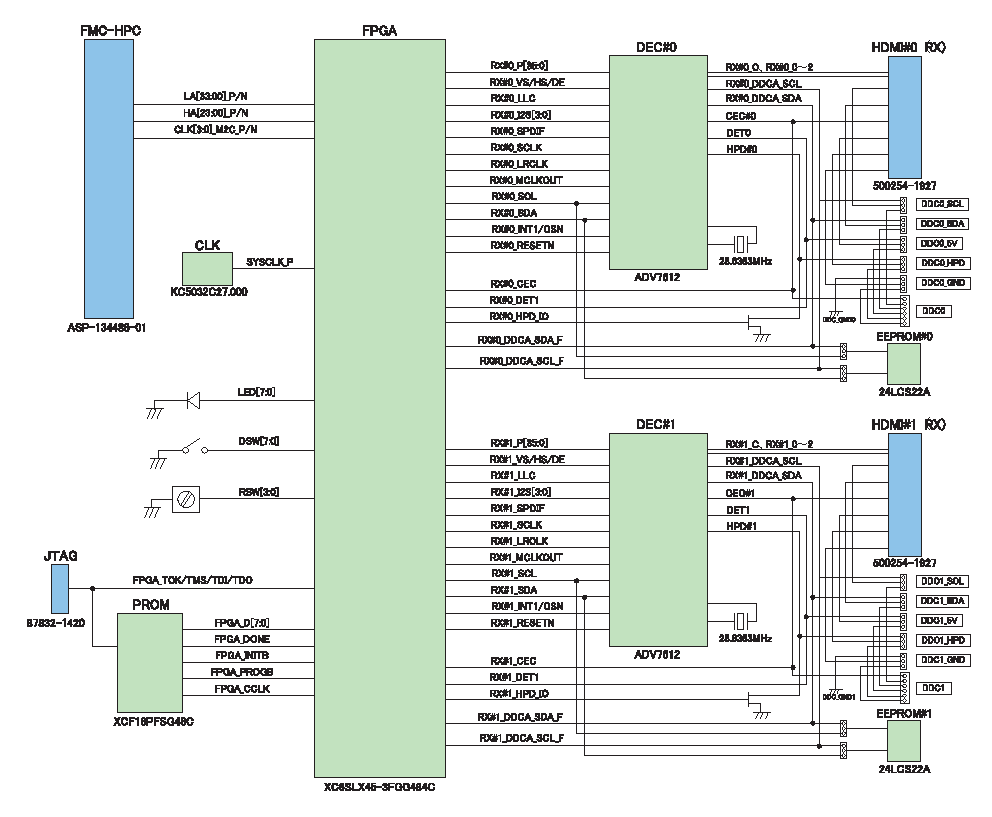
\includegraphics[width=1.0\textwidth]{diagramaBlocosRX_hdmi}
		\caption[Diagrama de blocos da placa HDMI RX]{Diagrama de blocos da placa HDMI RX (retirado de \cite{R009})}
		\label{fig:HDMIblocosRX}
	\end{center}
\end{figure}

Através de uma rápida observação deste diagrama é possível concluir que se pode dividir as suas principais funções em duas partes que passam a ser descritas nas próximas subsecções. 

\subsubsection{Receção do Sinal HDMI (ADV7612 para a FPGA localizada na placa)}
	
A receção do sinal HDMI é feita por um conector e usa um circuito integrado ADV7612BSWZ-P que recebe o sinal e retira do mesmo os sinais a serem passados para a FPGA localizada na placa HDMI. O recetor tem também uma memória EEPROM (\textit{Electrically Erasable Programmable Read-Only memory}) que é usada para guardar dados EDID.
	
\subsubsection{Interface com o conector FMC (da FPGA localizada na placa para o conector FMC)}

Após passarem pela FPGA integrada na placa, são passados os seguintes sinais presentes na tabela~\ref{table:HDMIdataRX} (para o caso em que a FPGA está configurada por omissão):

\begin{table}[h!]
	
			\centering
					\caption[Nomes dos pinos da interface FMC de TB-FMCH-HDMI2 RX]{Nomes dos pinos da interface FMC de TB-FMCH-HDMI2 RX (adaptada de \cite{R009})}
			\label{table:HDMIdataRX}
			\resizebox{\textwidth}{!}{ 
			
			\begin{tabular}{@{}lllll@{}}
			\toprule
			{\textbf{Nome do Pino}} & {\textbf{\textit{Input/Output}}} & {\textbf{FPGA para FMC}}& {\textbf{FMC para FPGA}}       \\ \midrule  
			CLK0\_M2C\_P         & \textit{Output}                & RX\#0\_LLC             & RX\#0 sinal LLC                \\ 
			CLK1\_M2C\_P         & \textit{Output}                & RX\#1\_LLC             & RX\#1 sinal LLC                \\ 
			LA00\_P\_CC          & \textit{Output}                & RX\#0\_VSYNC           & RX\#0\_VSYNC                   \\ 
			LA01\_P\_CC          & \textit{Output}                & RX\#0\_HSYNC           & RX\#0\_HSYNC                   \\ 
			LA02\_P              & \textit{Output}                & RX\#0\_DE              & RX\#0 data enable              \\ 
			LA03\_P a LA32\_P    & \textit{Output}                & RX\#0\_P0 a RX\#0\_P29 & RX\#0 dados de vídeo de 0 a 29 \\ 
			LA33\_P              & \textit{Input/Output}          & Não usado              & ---------                     \\ 
			CLK0\_M2C\_N         & \textit{Input/Output}          & Não usado              & ---------                     \\ 
			CLK1\_M2C\_N         & \textit{Input/Output}          & Não usado              & ---------                      \\ 
			LA00\_N\_CC          & \textit{Output}                & RX\#1\_VSYNC           & RX\#1\_VSYNC                   \\ 
			LA01\_N\_CC          & \textit{Output}                & RX\#1\_HSYNC           & RX\#1\_HSYNC                   \\ 
			LA02\_N              & \textit{Output}                & RX\#1\_DE              & RX\#1 data enable              \\ 
			LA03\_N a LA32\_N    & \textit{Output}                & RX\#1\_P0 a RX\#1\_P29 & RX\#1 dados de vídeo de 0 a 29 \\ 
			LA33\_P              & \textit{Input/Output}          & Não usado              & ---------                     \\ 
			CLK2\_M2C\_P         & \textit{Input/Output}          & Não usado              & ---------                     \\ 
			CLK3\_M2C\_P         & \textit{Input/Output}          & Não usado              & ---------                     \\ 
			HA00\_P a HA23\_P    & \textit{Input/Output}          & Não usado              & ---------                     \\ 
			CLK2\_M2C\_N         & \textit{Input/Output}          & Não usado              & ---------                     \\ 
			CLK3\_M2C\_N         & \textit{Input/Output}          & Não usado              & ---------                     \\ 
			HA00\_N a HA23\_N    & \textit{Input/Output}          & Não usado              & ---------                     \\ \bottomrule	
		\end{tabular}}		
		\centering

	\end{table}

Através da análise da tabela \ref{table:HDMIdataRX} e do diagrama de blocos da placa na figura \ref{fig:HDMIblocosRX} conclui-se que o integrado ADV7612 é capaz de colocar na sua saída vários sinais (tanto referentes à imagem como ao som), no entanto estes não são todos transmitidos para os conectores FMC. Isto deve-se à configuração presente na FPGA que determina os sinais a enviar para os conectores. Para além disto, através da leitura de \cite{R016} conclui-se que esta também configura alguns parâmetros do integrado ADV7612 que permitem que este transmita sinais num determinado formato e número de bits. 

Para esta configuração, são transmitidos para os conectores dados referentes à imagem e sinais de sincronização do mesmo. Os dados da imagem são enviados do recetor 0 entre os pinos LA03\_P a LA32\_P, e do recetor 1  entre LA03\_N a LA32\_P. O sinal “\textit{data enable}” sinaliza a chegada de dados e está ativo quando estão a ser transmitidos os sinais referentes a cada píxel. \textit{HSYNC} é um sinal que representa a sincronização horizontal e sincroniza o início da linha do dispositivo de destino com a imagem que o originou. Por outro lado, o sinal \textit{VSYNC} é a representação da sincronização vertical, que tem a mesma função que \textit{HSYNC}, certificando-se de que o dispositivo de destino começa no topo na imagem na altura correta.

Uma nota importante ainda sobre a passagem dos sinais através dos conectores FMC é que os dados provenientes da FPGA da placa para os conectores são amostrados no flanco negativo do sinal de relógio do vídeo. Assim, estes mesmos dados devem ser lidos no flanco positivo do sinal do relógio do lado da FPGA principal. A figura \ref{fig:HDMIamostragemRX}  ilustra esta situação.

\begin{figure}[h!]
	\begin{center}
		\leavevmode
		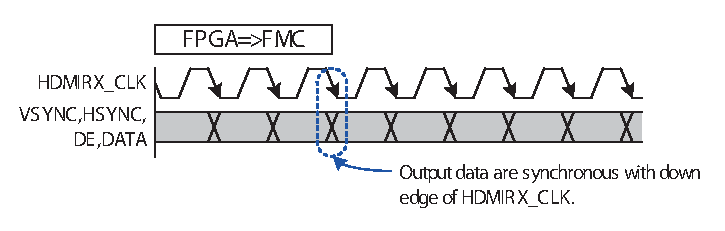
\includegraphics{amostragem_RX_vet}
		\caption[Amostragem dos dados provenientes da FPGA no recetor]{Amostragem dos dados provenientes da FPGA no recetor (retirada de \cite{R009})}
		\label{fig:HDMIamostragemRX}
	\end{center}
\end{figure}
 


\subsection{Transmissor}\label{subsec:TX} 

O diagrama de blocos do transmissor está representado na figura~\ref{fig:HDMIblocosTX}.

\begin{figure}[h!]
	\begin{center}
		\leavevmode
		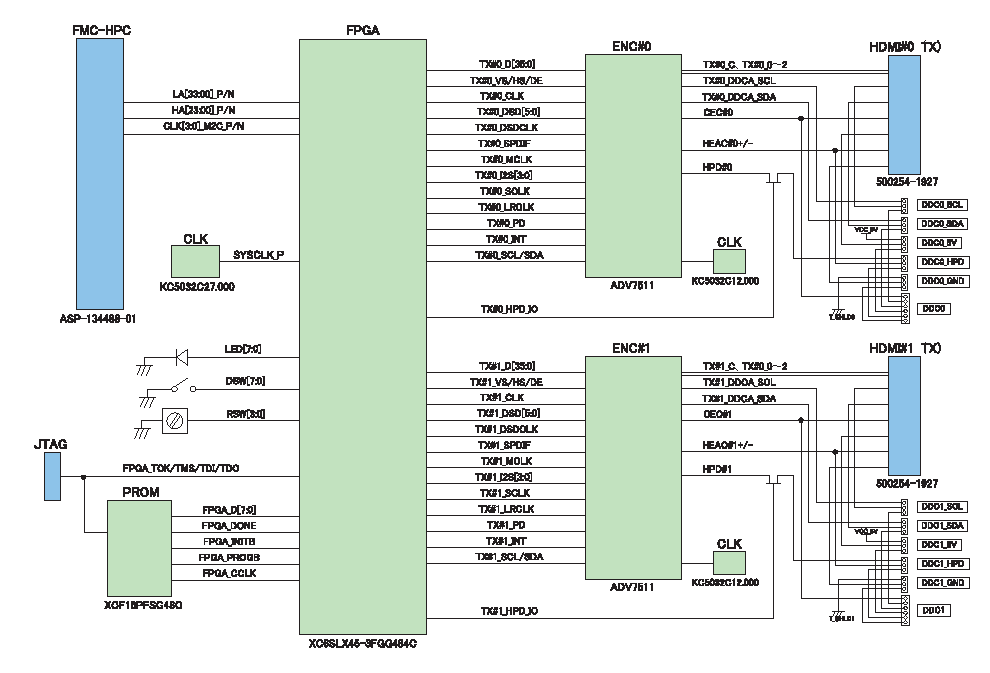
\includegraphics[width=1.0\textwidth]{diagramaBlocosTX_HDMI}
		\caption[Diagrama de blocos da placa HDMI TX]{Diagrama de blocos da placa HDMI TX (retirado de \cite{R009})}
		\label{fig:HDMIblocosTX}
	\end{center}
\end{figure}
Mais uma vez é possível dividir o diagrama em duas principais funções que passam a ser descritas.

\subsubsection{Interface com o conector FMC (do conector FMC para a FPGA localizada na placa)}
No caso do transmissor o processo é feito no sentido inverso, ou seja, os sinais são lidos dos conectores FMC da placa HDMI e são amostrados para a FPGA da mesma na transição de 0 para 1 do sinal de relógio do HDMI, tal como ilustra a figura \ref{fig:HDMIamostragemTX}. Estes são de seguida processados pela FPGA de maneira a serem enviados para o transmissor HDMI (ADV7511).

	\begin{figure}[h!]
	\begin{center}
		\leavevmode
		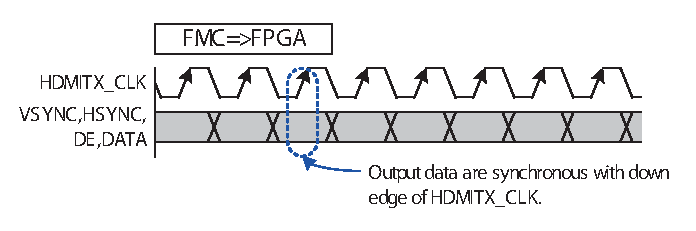
\includegraphics{amostragem_TX_vet}
		\caption[Amostragem dos dados provenientes do FMC no recetor]{Amostragem dos dados provenientes do FMC no recetor (retirada de \cite{R009})}
		\label{fig:HDMIamostragemTX}
	\end{center}
\end{figure}

Os sinais representados na tabela~\ref{table:HDMIdataTX} são equivalentes aos sinais presentes na tabela~\ref{table:HDMIdataRX}, mais uma vez com a placa configurada por omissão, e correspondem aos sinais que a placa transmissora deve receber através dos seus conectores.



\begin{table}[h!]
	
	\centering
	\caption[Nomes dos pinos da interface FMC de TB-FMCH-HDMI2 TX]{Nomes dos pinos da interface FMC de TB-FMCH-HDMI2 TX (adaptada de \cite{R009})}
	\label{table:HDMIdataTX}
	\resizebox{\textwidth}{!}{ 	
		\begin{tabular}{@{}lllll@{}}
			\toprule
			\textbf{Nome do pino} & \textbf{Input/0utput} & \textbf{FMC para FPGA} & \textbf{FPGA para TX}          \\ \midrule
			CLK0\_M2C\_P         & Input                 & TX\#0\_DCLK            & TX\#0 sinal DCLK               \\ 
			CLK1\_M2C\_P         & Input/Output          & Não usado              & ----------                     \\ 
			LA00\_P\_CC          & Input                 & TX\#0\_VSYNC           & TX\#0\_VSYNC                   \\ 
			LA01\_P\_CC          & Input                 & TX\#0\_HSYNC           & TX\#0\_HSYNC                   \\ 
			LA02\_P              & Input                 & TX\#0\_DE              & TX\#0 data enable              \\ 
			LA03\_P a LA32\_P    & Input                 & TX\#0\_D0 a TX\#0\_D29 & TX\#0 dados de vídeo de 0 a 29 \\ 
			LA33\_P              & Input/Output          & Não usado              & ----------                     \\ 
			CLK0\_M2C\_N         & Input                 & TX\#1\_DCLK            & TX\#0 sinal DCLK               \\ 
			CLK1\_M2C\_N         & Input/Output          & Não usado              & ----------                     \\ 
			LA00\_N\_CC          & Input                 & TX\#1\_VSYNC           & TX\#1\_VSYNC                   \\ 
			LA01\_N\_CC          & Input                 & TX\#1\_HSYNC           & TX\#1\_HSYNC                   \\ 
			LA02\_N              & Output                & TX\#1\_DE              & TX\#1 data enable              \\ 
			LA03\_N a LA32\_N    & Output                & TX\#1\_D0 a TX\#1\_D9  & TX\#1 dados de vídeo de 0 a 29 \\ 
			LA33\_P              & Input/Output          & Não usado              & ----------                     \\ 
			CLK2\_M2C\_P         & Input/Output          & Não usado              & ----------                     \\ 
			CLK3\_M2C\_P         & Input/Output          & Não usado              & ----------                     \\ 
			HA00\_P a HA23\_P    & Input/Output          & Não usado              & ----------                     \\ 
			CLK2\_M2C\_N         & Input/Output          & Não usado              & ----------                     \\ 
			CLK3\_M2C\_N         & Input/Output          & Não usado              & ----------                     \\ 
			HA00\_N a HA23\_N    & Input/Output          & Não usado              & ----------                     \\ \bottomrule
		\end{tabular}}
	\end{table}
	
\subsubsection{Transmissor HDMI (da FPGA localizada na placa para ADV7511)}

Os sinais recebidos são processados pela FPGA de maneira a enviá-los para o bloco ADV7511 localizado na placa. Através da análise dos documentos \cite{R017} e \cite{R018} conclui-se que, para além dos dados de imagem e os seus sinais de controlo, são também enviados para o integrado ADV7511 sinais que indicam as características de trasnmissão de entrada e saída. De seguida, o ADV7511 converte o sinal para o poder enviar através do cabo HDMI para o dispositivo final. 



%\subsubsection{Conexão DDC}\label{subsubsec:DDCconexao} 
%
%Para esta configuração da placa, são suportadas dois tipos de conexão DDC que passam a ser descritas.
%
%\begin{enumerate}
%	\item \textbf{Conexão Normal}
%	
%	\hspace{1.0em}Nesta configuração a comunicação DDC realiza-se normalmente entre o recetor e o transmissor HDMI, tal como ilustra a figura~\ref{fig:DDCnormal} na página~\pageref{fig:DDCnormal}. Existe um canal especifico para esta conexão que é recebido através do conector HDMI e enviado juntamente com os outros tipos de dados.
%
%	\begin{figure}[h!]
%		\begin{center}
%			\leavevmode
%			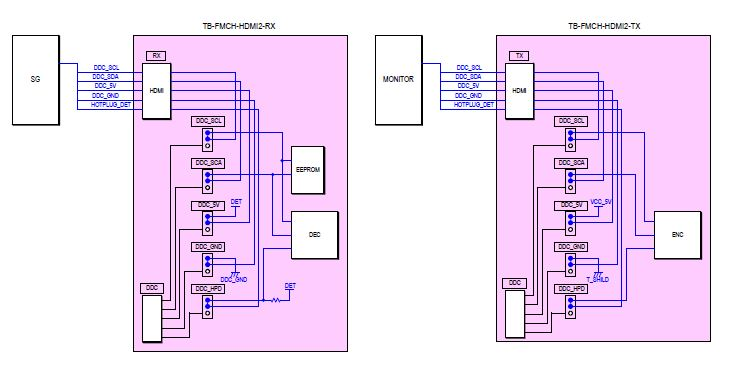
\includegraphics[width=1.0\textwidth]{DDCnormal}
%			\caption{Configuração DDC normal, retirada de \cite{R009}}
%			\label{fig:DDCnormal}
%		\end{center}
%	\end{figure}
%	
%	\item \textbf{Conexão "\textit{through}"}
%	
%	\hspace{1.0em}Este tipo de conexão faz uma ligação direta do canal DDC entre o recetor e o transmissor inibindo a comunicação normal deste canal. Para fazer esta conexão é necessário um cabo DDC e fazer as conexões corretas. Esta situação está ilustrada na figura~\ref{fig:DDCthrough} na página~\pageref{fig:DDCthrough}.
%	
%		\begin{figure}[h!]
%		\begin{center}
%			\leavevmode
%			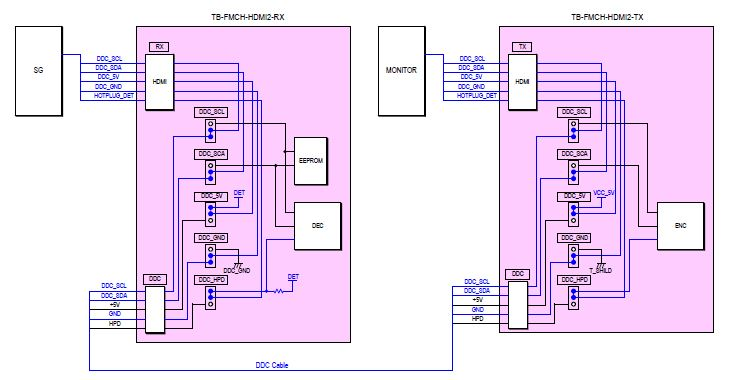
\includegraphics[width=1.0\textwidth]{DDCthrough}
%			\caption{Configuração DDC “\textit{through}”, retirada de \cite{R009}}
%			\label{fig:DDCthrough}
%		\end{center}
%	\end{figure}
%	
%	\hspace{1.0em}Este tipo de configuração poderá ser utilizada numa fase inicial do projeto a ser realizado, visto que não exige comunicação bidirecional através dos transcetores (onde os restantes sinais serão transmitidos), e como tal vem facilitar a comunicação entre dispositivo de origem e de destino.
%\end{enumerate}

%\section{Conexão de alta velocidade em série -> NOVO SUB-CAPITULO} \label{sec:conexaoSerie_new}
%
%A comunicação de dados de alta velocidade pode ser efetuada tanto em série como em paralelo, sendo que cada uma tem as suas devidas implicações. No caso das comunicações em paralelo é possivel atingir uma velocidade de comuncação maior, no entanto tem um custo mais elevado devido à necessidade de mais recursos físicos. Para além de um custo maior apresentam também 



\section{Conexão de alta velocidade em série} \label{sec:conexaoSerie}

Nesta secção é abordado o tema de comunicação em série em alta velocidade, desde as suas vantagens e desvantagens até tipos de arquiteturas habitualmente utilizados.

\subsection{Comunicações em paralelo VS comunicações em série}

Desde sempre que tanto a comunicação em série como em paralelo têm vindo a ser utilizadas para as diferentes aplicações que envolvem a transmissão de dados entre módulos, e nesta subsecção são abordadas as diferentes características de cada um. A comunicação de dados em paralelo é utilizada para comunicações relativamente curtas pelo facto de ser mais simples e não trazer tantas implicações. Olhando para um exemplo em concreto deste projeto: a comunicação entre as placas HDMI e a FPGA VC7203 é feita em paralelo através dos conectores FMC, tal como explicado em \ref{subsec:HDMIconexao}, porque é uma distância bastante curta e não envolve preocupações no que toca a dobrar ou triplicar a frequência de transmissão e vice-versa. Afinal, para transmitir um determinado número de dados em série é necessário multiplicar esse número de dados pela frequência de transmissão em paralelo do lado do transmissor, e do lado do recetor é necessário lidar com eventuais desalinhamentos. 

Quando as comunicações em paralelo começaram a ser utilizadas a distâncias maiores e a ser também necessário uma velocidade de comunicação maior, começaram a surgir  mais problemas relativamente ao uso desta forma de transmissão. Apesar de, segundo \cite{R032}, terem sido aplicados métodos que viessem melhorar o desempenho destas comunicações em termos de velocidade, como por exemplo, a sinalização diferencial que veio aumentar a mesma, existem ainda bastantes desvantagens segundo \cite{R012}. Há uma  desvantagem que se torna bastante óbvia de constatar que é o custo: ter uma ligação em série com um cabo é muito menos dispendioso do que ter 400 cabos (no caso da transmissão entre as placas HDMI e a FPGA) para ter uma ligação em paralelo. Para além disto, existem mais três problemas também apontados por \cite{R012} : \textit{clock skew}, \textit{data skew} e \textit{crosstalk}. \textit{Clock} e \textit{data skew} tratam-se de pequenos desvios na chegada ao recetor dos dados e dos sinais de relógio, isto porque nem todos são transmitidos exatamente à mesma velocidade e como tal podem provocar pequenos atrasos. Apesar de serem pequenos, podem vir a causar problemas visto que a velocidade de transmissão é bastante alta. Segundo este mesmo autor, existem já técnicas capazes de corrigir estes atrasos relativamente ao sinal de relógio (devido à sua periocidade), e a correcção dos dados também é possível, no entanto é muito mais problemática. A \textit{crosstalk} trata-se de uma interferência entre cabos adjacentes, inerente à transmissão, que se torna ainda mais problemática com o aumento dos mesmos.

%Falar das vantagens de usar comunicação em série
Estas razões, entre outras, têm vindo a motivar o desuso das comunicações em paralelo para transmissões de alta velocidade. Em \cite{R032} são expostas algumas das razões para usar as ligações em série para tal efeito. O autor menciona o facto da utilização de menos pinos para uma maior largura de banda, o que faz com que o custo da transmissão baixe consideravelmente. Este autor considera também um problema das transmissões em paralelo que não acontece em série: as consequências das constantes alternâncias das saídas. Isto é, numa ligação em paralelo o mais provável é que todas as saídas estejam a alternar constantemente e, como tal, esta alternância na massa acaba por criar ruído que é propagado na ligação. Claro que é possível resolver este problema aplicando sinalização diferencial aos sinais transmitidos, mas em contrapartida aumenta o número de pinos necessários, aumentando por isso o custo da ligação.

%Desvantagens de usar comunicação em série
Aparentemente, torna-se óbvio que as ligações em série devem ser usadas para este efeito uma vez que só acartam consigo vantagens, no entanto é necessário ter com consideração as desvantagens desta utilização. 

Logo à partida o primeiro problema que rapidamente o autor de \cite{R032} constata é a integridade do sinal, isto é, é expectável que para garantir a integridade do sinal será necessário recorrer a mais lógica que o garanta. Para além disso, também será de esperar que este tipo de comunicaçãos exiga placas, cabos e conectores de alta velocidade que são mais caros. E claro, uma vez que estas comunicações trabalham a uma cadência bastante elevada também é de esperar que seja necessário fazer simulações digitais em bases de tempo mais pequenas o que pode trazer algumas complicações.
%Problemas na integridade do sinal
%Também podemos esperar para pagar mais por placas de PC controladas por impedância, conectores e cabos de alta velocidade.

Em conclusão, e tal como o autor de \cite{R032} menciona, hoje em dia a utilização de ligações em série já não são utilizadas apenas na indústria das telecomunicações mas acaba por ser transversal a outras tantas que a usam. O autor remata ainda que o futuro da eletrónica passa por comunicações em série.
%O autor de \cite{R032} menciona que hoje em dia este tipo de comunicações é usada não so na indústria das telecomunicações mas também numa vasta variedade de seccções e remata ainda que o futuro da eletrónica passa por comunicações em série. Este autor refere ainda que este tipo de comunicações pode vir a trazer vantagens em ligações \textit{chip-to-chip}
%Falar de onde e que podem ser utilizadas este tipo de comunicações

%Estes motivos apresentados entre outros têm vindo a motivar o uso de transmissão em série para longas distâncias a alta velocidade. O autor de \cite{R012} relembra ainda que as transmissões em paralelo não caíram nem nunca cairão em desuso uma vez que são eficientes em transmissões internas entre circuitos integrados e comunicações "\textit{chip to chip}" relativamente curtas, como é utilizado neste projeto para a comunicação entre a placa HDMI e a FPGA VC7203, para permitir uma taxa de transmissão elevada e ao mesmo tempo um processamento de sinal rápido.


%Maximum Data Flow
%Pin Count
%EMI
%Cost


%A comunicação de dados de alta velocidade pode ser efetuada tanto em série como em paralelo, no entanto cada uma tem as suas implicações. No caso das comunicações em paralelo permitem uma velocidade de comunicação maior, em contrapartida tem um custo mais elevado devido à necessidade de mais recursos físicos e apresenta ainda problemas no que toca à diferença de tempos de chegada de dados e sinais de relógio (visto que estes podem chegar a tempos diferentes) e também no que toca à interferência entre canais. 
%
%Desta maneira, segundo \cite{R012}, comunicações em série têm vindo a substituir as comunicações em paralelo em ligações de alta velocidade. Apesar disso, as comunicações realizadas dentro dos circuitos integrados são normalmente realizadas em paralelo, visto que permite maior rapidez de comunicação, e como tal é necessário a utilização de serializadores e deserializadores no sentido de transformar os dados nos diferentes domínios em que são utilizados.

\subsection{Considerações sobre arquiteturas de transmissão de dados em série} \label{serial_theory}
Nesta subsecção são apresentadas considerações que devem ser tomadas quando se trata de implementar uma arquitetura que permita enviar dados em série a alta velocidade.
\subsubsection*{Arquitetura de serializadores e deserializadores de alta velocidade}

No projeto desenvolvido lida-se com sinais provenientes da fonte HDMI em paralelo e para que seja possível transmiti-los em série a alta velocidade é necessário implementar um arquitetura capaz de lidar com este processo de conversão. Nesta subsecção são abordadas algumas técnicas de implementação de serializadores e deserializadores, as suas características e cuidados na sua implementação.

Na figura \ref{fig:arquiteturaSER} é apresentada uma simples arquitetura de um serializador e deserializador proposto pelo autor de \cite{R032}. A figura ilustra um diagrama de blocos, em que cada bloco possui uma determinada função para se obter uma conversão de dados paralelo para série e vice-versa.

\begin{figure}[h!]
	\begin{center}
		\leavevmode
		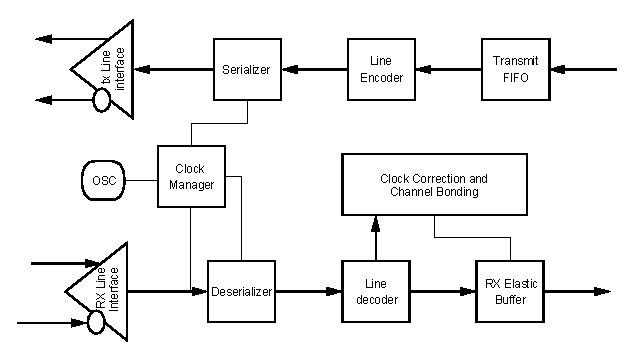
\includegraphics[width=1.0\textwidth]{ser_des}
		\caption[Arquitetura simples de um serializador e deserializador]{Arquitetura simples de um serializador e deserializador (retirada de \cite{R032})}
		\label{fig:arquiteturaSER}
	\end{center}
\end{figure}

As funções de cada bloco do diagrama do serializador apresentado passam a ser brevemente descritas:

\begin{itemize}
	\item \textbf{\textit{Transmit FIFO (First in, First out):}} Trata-se de uma memória FIFO que guarda os dados em paralelo antes destes serem enviados para o resto da arquitetura. No diagrama poderia também estar representa uma fonte direta de sinais em paralelo (como é o caso deste projeto).
	
	\item\textbf{\textit{Line Enconder:}} Este bloco trata-se de um  bloco opcional, e nem em todas as arquiteturas de serializadores/deserializadores está presente. Este bloco codifica os dados que recebe para um formato \textit{"line-friendly"} \footnote{é o termo usado pelo autor de \cite{R032}}. Trata-se de um formato que ajuda o recetor a recuperar os sinais da dados e relógio, normalmente envolvendo a eliminação de longas tramas de zeros ou uns, de maneira a garantir que há um equilíbrio entre o número de uns e zeros numa trama.
	
	\item \textbf{\textit{Serializer:}} Tal como o nome indica este é um bloco que serializa os dados que recebe, ou seja, quando recebe um determinado número de dados em paralelo (x dados) a uma determinada cadência (frequência y), transforma-o num \textit{stream} de dados a uma taxa de x multiplicado por y.
	 
	\item \textbf{\textit{TX Line Interface:}} Este bloco acaba por ser a interface final do serializador com o cabo físico, e geralmente também lhe são aplicados determinados processos que permitem a melhor recuperação do sinal do lado do recetor.
\end{itemize}

Por outro lado, o deserializador tem de fazer todo o processo inverso que o bloco serializador faz. As funções de cada bloco passam a ser brevemente descritas.

\begin{itemize}
	\item \textbf{\textit{RX Line Interface:}} É a interface do deserializador com o cabo físico. Já pode incluir alguma equalização do sinal passiva ou ativa.
	\item\textbf{\textit{Deserializer:}} Converte os dados em série que recebe a uma cadência de x multiplicado por y, em x dados paralelo a uma cadência de y.
	\item \textbf{\textit{Line Decoder:}} Descodifica os dados recebidos, se tal processo foi realizado do lado do transmissor.
	\item \textbf{\textit{RX Elastic Buffer:}} Este bloco permite o alinhamento dos dados recebidos para os repectivos limites. Tal pode ser feito automaticamente ou recorrer-se a palavras de alinhamento, também chamadas de "vírgulas".
	\item \textbf{\textit{Clock Correction and Channel Bonding:}} Este bloco permite que haja correção entre as diferenças de sinais de relógio, e ainda correção de atrasos entre diferentes canais (caso haja transmissão em vários canais). 
\end{itemize}

Existe ainda um bloco que é comum tanto ao serializador como ao deserializador que é o \textbf{\textit{Clock Manager}} que essencialmente é responsável pelos diversos processos que os sinais de relógio necessitam: desde multiplicações de frequências, divisões e até mesmo recuperação do mesmo.

Esta arquitetura aqui apresentada acaba por expor os blocos essenciais para o correto funcionamento de um serializador e deserializador, no entanto existem outras características que podem ser adicionadas: desde os diferentes tipos de codificações possíveis, até códigos detetores e corretores de erros que podem ser adicionados à arquitetura.

%\begin{figure}[h!]
%	\begin{center}
%		\leavevmode
%		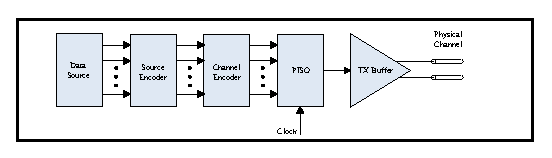
\includegraphics[width=1.0\textwidth]{ser_arq_vet}
%		\caption{Arquitetura simples de um serializador, retirada de \cite{R012}}
%		\label{fig:arquiteturaSER}
%	\end{center}
%\end{figure}



%\begin{figure}[h!]
%	\begin{center}
%		\leavevmode
%		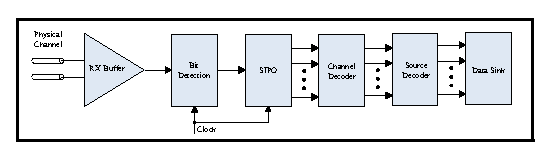
\includegraphics[width=1.0\textwidth]{des_arq_vet}
%		\caption{Arquitetura simples de um deserializador, retirada de \cite{R012}}
%		\label{fig:arquiteturaDES}
%	\end{center}
%\end{figure}

%\begin{itemize}
%	\item Chegada do sinal em paralelo ao bloco “\textit{data source}”, que corresponde à chegada dos dados em paralelo a serem posteriormente transmitidos.
%	\item Codificação da fonte (\textit{source enconding}) é bloco que se segue nesta arquitetura e inclui construção de tramas, sincronização de padrões e ainda FEC \footnote{\textit{Foward Error Correction} é uma técnica que permite o controlo de erros na transmissão de dados.}.
%	\item O bloco seguinte da arquitetura corresponde à codificação de canal, que é realizada de maneira a que o sinal a ser transmitido consiga um melhor desempenho no que toca a deteção de bits no recetor.
%	\item De seguida, o sinal codificado é enviado para o bloco PISO (\textit{parallel input - serial output)} e de onde sai um sinal em série dos dados a serem enviados.
%	\item Finalmente estes dados são enviados para o \textit{buffer} para que possam ser devidamente convertidos em sinais elétricos ou pulsos óticos para que de seguida sejam transmitidos pela camada física. 
%	\item Em alguns casos um equalizador (\textit{pre-emphasis}) para corrigir alguns erros que possam acontecer no canal em ligações de alta velocidade é utilizado. Erros podem acontecer por diversos motivos, entre os quais: a dependência da atenuação e da dispersão relativamente à frequência, interferências e ruído.
%\end{itemize}
%
%O deserializador proposto segue a mesma estrutura que o serializador fazendo, no entanto, o processo inverso.

%\subsubsection*{Considerações na implementação deste tipo de arquitetura}
%Em \cite{R012} são apontados os principais desafios na implementação deste tipo de arquitetura que passarão a ser descritos brevemente e que têm de ter sidos em conta aquando a sua implementação.

\subsubsection*{Restrições na utilização de circuitos de serializadores e deserializadores} \label{subsub:restricoes_circuitos}
	
Quando se passa para a implementação de serializadores e deserializadores é necessário ter em conta algumas considerações relativamente aos circuitos utilizados. Segundo \cite{R012}, logo à partida existem grandes restrições no que toca aos circuitos utilizados nestes tipos de arquiteturas. Isto porque os sinais recebidos em paralelo são sinais digitais, contudo quando estes sinais passam pelo canal de transmissão sofrem distorções e também lhes é adicionado ruído, o que leva a que o sinal recebido do lado do recetor seja um sinal analógico e que necessite de ser tratado como tal. A sua recuperação tem de ser então baseada na regeneração correta do sinal de relógio e também na amostragem apropriada. 
	
Ao mesmo tempo, este tipo de dispositivos são normalmente um subsistema de um sistema grande e usados em dispositivos portáteis, e como tal precisam de ter um baixo consumo de energia. Assim sendo, um dos primeiros grandes desafios desta implementação de serializador/deserializador, segundo \cite{R012}, é conseguir implementar circuitos digitais de alta velocidade e ao mesmo tempo possuem um baixo consumo de potência. Este mesmo autor apresenta duas principais técnicas utilizadas para alcançar tais objetivos que passam pela utilização de lógica CMOS (\textit{Complementary metal-oxide-semiconductor}) que permitem a utilização a alta velocidade com baixo consumo de potência. 
	
Outro requisito crítico na implementação deste tipo de arquiteturas é também a adaptação das impedâncias características do \textit{buffer} (de transmissão e receção) com a impedância característica da linha onde é transmitido o sinal. Isto porque, caso estas não estejam adaptadas ocorrerão reflexões no lado do transmissor ou do recetor (consoante a desadaptação) que não permitem a transmissão da potência total do sinal. No entanto, este requisito requer um grande consumo de potência, pois na prática os canais de transmissão têm uma impedância muito baixa. 


\subsubsection*{Codificação dos sinais e sua importância} \label{subsub:cod_impor}

O bloco de codificação de sinais insere-se nesta arquitetura do transmissor devido à sua importância relativamente à recuperação dos dados do lado do recetor. Estes blocos modificam os sinais para um formato que permite ao recetor recuperar os sinais de relógio mais facilmente, garantindo que existe um número suficiente de transições entre zero e um. Segundo \cite{R032}, este bloco, para além de fazer o que já foi descrito garante que existe um balanço entre zeros e uns na linha de transmissão (\textit{Direct Current Balance} - DC \textit{Balance}) e opcionalmente pode também implementar mecanismos de correção de sinal de relógio, sincronização de blocos e eventuais sinalização de canais (quando é usado mais do que um canal físico na transmissão).

%Codificação 8B/10B
Ainda segundo o autor de \cite{R032}, um dos esquemas de codificação e descodificação mais utilizados em diversos protocolos é 8B/10B. Este tipo de codificação converte palavras de 8 bits em 10 bits garantindo um número suficiente de transições entre zeros e uns nas palavras codificadas. Este mecanismo irá garantir que o sinal de relógio será corretamente recuperado do lado do recetor. Na tabela \ref{table:cod_8b_10b_ex} é possível encontrar dois exemplos de codificação de palavras de 8 bits em 10 bits. Note-se que palavras que não apresentam transições entre zero e um (no caso da primeira linha da tabela) ou poucas (no caso da segunda linha da tabela) passam a ter transições suficientes para que o sinal de relógio possa ser recuperado do lado do recetor.

\begin{table}[h!]
	\centering
	\caption[Exemplo de codificação 8B/10B]{Exemplo de codificação 8B/10B (retirada de \cite{R032})}
	\label{table:cod_8b_10b_ex}
	\begin{tabular}{@{}ll@{}}
		\toprule
		\multicolumn{1}{c}{\textbf{Palavra de 8 bits}} & \multicolumn{1}{c}{\textbf{Símbolo de 10 bits}} \\ \midrule
		00000000                                       & 1001110100                                      \\
		00000001                                       & 0111010100                                      \\ \bottomrule
	\end{tabular}
	

\end{table}

%Importância da disparidade e DC Balance
Este método de codificação garante que existe um balanço entre o número de zeros e uns na linha de transmissão de uma maneira particular, chamada disparidade. Afinal, a maneira mais fácil de garantir este balanço seria limitar os números de zeros e uns em cada palavra (5 zeros e 5 uns), que por acaso são os exemplos apresentados na tabela \ref{table:cod_8b_10b_ex}. Contudo esta restrição viria limitar o número de palavras de 10 bits possíveis de obter. Em vez disso, este método utiliza dois símbolos para palavra codificada. Isto é, para uma palavra de 8 bits codifica de duas maneiras possíveis em que, geralmente, uma tem 6 zeros e 4 uns e a outra tem 4 zeros e 6 uns. Essencialmente, para cada palavra de 8 bits há duas possibilidades de codificação e durante a transmissão das palavras a seleção é feita com base na necessidade de balanço de zeros e uns na linha. Geralmente os símbolos são reconhecidos por + e -.

Outra vantagem da utilização deste tipo de codificação tem a ver com a deteção de erros do lado do recetor. Isto é,  este monitoriza o balanço de zeros e uns tendo em conta a disparidade e caso haja alguma violação nestas regras então o recetor é capaz de detetar a ocorrência de erros.

\begin{table}[h!]
		\caption[Exemplo de palavras de 8 bits codificadas em 8B/10B]{Exemplo de palavras de 8 bits codificadas em 8B/10B (retirada de \cite{R032})}
	\label{table:exemple_trans}
	\centering
	\resizebox{\textwidth}{!}{%
	\begin{tabular}{@{}llll@{}}
		\toprule
		\multicolumn{1}{c}{\textbf{Hexadecimal}} & \multicolumn{1}{c}{\textbf{Palavra de 8 bits}} & \multicolumn{1}{c}{\textbf{Símbolo de 10 bits (-)}} & \multicolumn{1}{c}{\textbf{Símbolo de 10 bits (+)}} \\ \midrule
		EA                                       & 11101010                                       & 0101011110                                          & 0101010001                                          \\
		FF                                       & 11111111                                       & 1010110001                                          & 0101001110                                          \\
		A4                                       & 10100100                                       & 1101011010                                          & 0010101010                                          \\ \bottomrule
	\end{tabular}
	}

\end{table}

Na tabela \ref{table:exemple_trans} são apresentadas três palavras de 8 bits codificadas nas suas duas possibilidades. A palavra apresentada na 1ª linha, EA em hexadecimal, na sua codificação negativa apresenta 6 uns e 4 zeros, contudo na sua forma positiva apresenta 4 uns e 6 zeros. O mesmo acontece com a palavra apresentada na última linha. No entanto a palavra representada na 2ª linha apresenta o mesmo número de zeros e uns em ambos os formatos. Se hipoteticamente fosse necessário transmitir estas palavras seguidas, o codificador teria em atenção o balanço entre zeros e uns na linha de transmissão aquando a transmissão da palavra EA e A4 para que o mesmo fosse garantido.
 
\subsubsection*{Alinhamento da transmissão} \label{subsub:alinhamento}
Uma função importante do deserializador, segundo o autor de \cite{R032} é o alinhamento dos dados que chegam em série. Por outras palavras, é importante que o deserializador reconheça os limites de uma determinada palavra transmitida. Para esse efeito são usados uns símbolos especiais que a codificação 8B/10B disponibiliza. Segundo \cite{R032}, este tipo de codificação dispõe de 12 símbolos que se codificam em 12 símbolos de controlo geralmente conhecidos por por \textit{K-characters}. Estes são geralmente usados para alinhamento e controlo devido às suas particulares características. Esses mesmos símbolos são apresentados na tabela \ref{table:caracteres_especiais_8b10b}.

\begin{table}[h!]
	\centering
		\caption[Símbolos de controlo especificos da codificação 8B/10B]{Símbolos de controlo específicos da codificação 8B/10B (retirada de \cite{R032})}
	\label{table:caracteres_especiais_8b10b}
	\resizebox{\textwidth}{!}{%
		\begin{tabular}{@{}lllll@{}}
			\toprule
			\multicolumn{1}{c}{\textbf{Nome}} & \multicolumn{1}{c}{\textbf{Hexadecimal}} & \multicolumn{1}{c}{\textbf{Palavra de 8 bits}} & \multicolumn{1}{c}{\textbf{Símbolo de 10 bits (+)}} & \multicolumn{1}{c}{\textbf{Símbolo de 10 bits (-)}} \\ \midrule
			K28.0                             & 1C                                       & 00011100                                       & 0011110100                                          & 1100001011                                          \\
			K28.1                             & 3C                                       & 00111100                                       & 0011111001                                          & 1100000110                                          \\
			K28.2                             & 5C                                       & 01011100                                       & 0011110101                                          & 1100001010                                          \\
			K28.3                             & 7C                                       & 01111100                                       & 0011110011                                          & 1100001100                                          \\
			K28.4                             & 9C                                       & 10011100                                       & 0011110010                                          & 1100001101                                          \\
			K28.5                             & BC                                       & 10111100                                       & 0011111010                                          & 1100000101                                          \\
			K28.6                             & DC                                       & 11011100                                       & 0011110110                                          & 1100001001                                          \\
			K28.7                             & FC                                       & 11111100                                       & 0011111000                                          & 1100000111                                          \\
			K23.7                             & F7                                       & 11110111                                       & 1110101000                                          & 0001010111                                          \\
			K27.7                             & FB                                       & 11111011                                       & 1101101000                                          & 0010010111                                          \\
			K29.7                             & FD                                       & 11111101                                       & 1011101000                                          & 0100010111                                          \\
			K30.7                             & FE                                       & 11111110                                       & 0111101000                                          & 1000010111                                          \\ \bottomrule
		\end{tabular}%
	}
\end{table}

Para conseguir alinhar, o recetor procura por uma palavra de alinhamento, conhecida por "\textit{comma}" (vírgula em português), e quando a encontra repõe os limites de alinhamento das palavras. Como esta procura é contínua, a partir da primeira deteção todas as palavras de alinhamento que forem detetadas encontrarão o alinhamento já feito. O valor deste símbolo que delimita as palavras (\textit{comma}) pode à partida ser definido no transcetor, contudo por vezes pode vir já pré-definido. 

%\begin{figure}[h!]
%	\begin{center}
%		\leavevmode
%		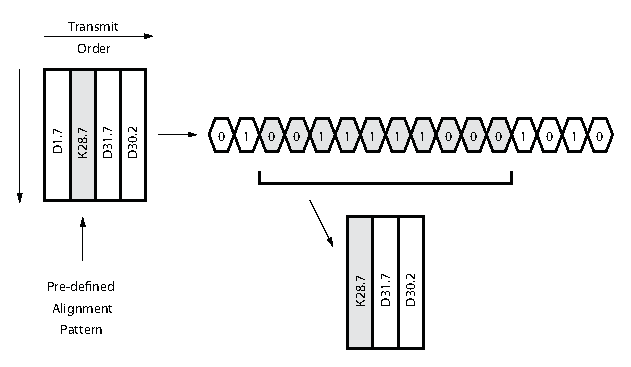
\includegraphics[width=0.8\textwidth]{align_vet}
%		\caption{Exemplo de transmissão de dados codificados em 8B/10B, retirada de \cite{R032}}
%		\label{fig:alinhamento_8B_10B}
%	\end{center}
%\end{figure}

\begin{figure}[h!]
	\begin{center}
		\leavevmode
		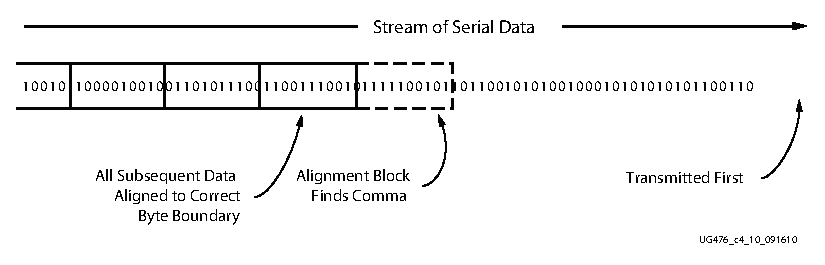
\includegraphics[width=1.0\textwidth]{serial_align_vet}
		\caption[Ilustração do alinhamento em série quando encontrada a \textit{comma}]{Ilustração do alinhamento em série quando encontrada a \textit{comma} (retirada de \cite{R011})}
		\label{fig:alinhamento_serie}
	\end{center}
\end{figure}

A figura \ref{fig:alinhamento_serie} ilustra o que acontece ao \textit{stream} de bits que chegam ao recetor em série. Aquando da deteção da palavra de alinhamento todos os dados que são retirados daí para a frente já se encontram alinhados pelo delimitação da palavra. Na figura \ref{fig:alinhamento_paralelo} é ilustrado o mesmo exemplo mas em paralelo, para melhor entendimento do processo de alinhamento. Todos os dados recebidos no recetor antes da palavra de alinhamento são considerados dados não alinhados.

\begin{figure}[h!]
	\begin{center}
		\leavevmode
		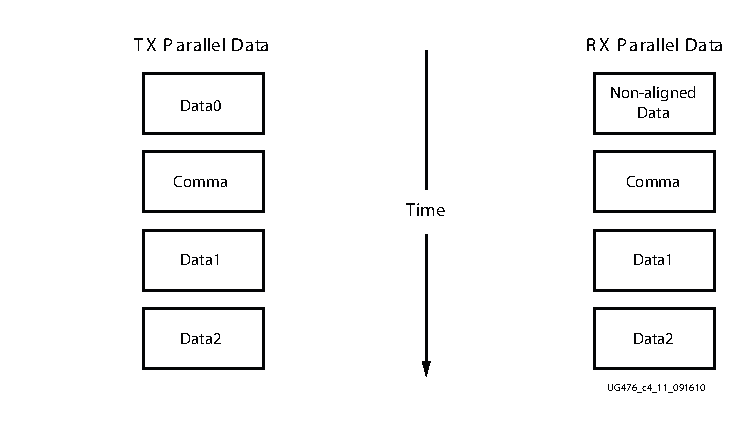
\includegraphics[width=1.0\textwidth]{paralel_align}
		\caption[Ilustração do alinhamento em paralelo quando encontrada a \textit{comma}]{Ilustração do alinhamento em paralelo quando encontrada a \textit{comma} (retirada de \cite{R011})}
		\label{fig:alinhamento_paralelo}
	\end{center}
\end{figure}

Tal como o autor de \cite{R032} menciona, a palavra de alinhamento deve ser única e diferenciável de todos os outros dados que possam ser transmitidos. Este mesmo autor sugere que os símbolos especiais \textit{K-characters} mencionados na tabela \ref{table:caracteres_especiais_8b10b} sejam utilizados para tal efeito, sendo que os mais adequados são o K28.1, K28.5 ou K28.7, pois todos têm um padrão inicial de 7 bits de 1100000, que apenas é encontrado nestes símbolos. Tal padrão não é encontrado em nenhuma outra sequência ordenada de dados ou em qualquer outro \textit{K-character}, e por isso é ideal para o alinhamento. Este autor reforça ainda que quando um protocolo de comunicação está a ser construído, como é o caso deste projeto, a maneira mais segura é "pedir emprestado" este tipo de sinais de controlo a protocolos bem conhecidos.



\subsubsection*{PISO (\textit{Parallel input – serial output}) e SIPO (\textit{serial input – parallel output})}

Os blocos de serialização e deserialização da arquitetura têm uma grande importância no correto funcionamento de toda a arquitetura, isto porque, tal como o nome indica, estes convertem os dados em paralelo em série e vice-versa. Tal como já foi referido anteriormente, o serializador recebe N dados a uma frequência de X, e transmite esses N dados a uma frequência de X*N. Por outro lado o deserializador, reduz a frequência dos dados, convertendo-os em paralelo, para de seguida ser enviada para o resto da arquitetura para processamento desses mesmos dados. Por isso, é necessário tomar em atenção diversas características quanto à escolha destas arquieturas, tais como a sua latência.

O autor de \cite{R012} propõe três tipos de arquiteturas para este tipo de bloco que são apresentadas na figura \ref{fig:PISO-SIPO} cujas vantagens e desvantagens passam de seguida a ser expostas.


	\begin{figure}[h!]
	\begin{center}
		\leavevmode
		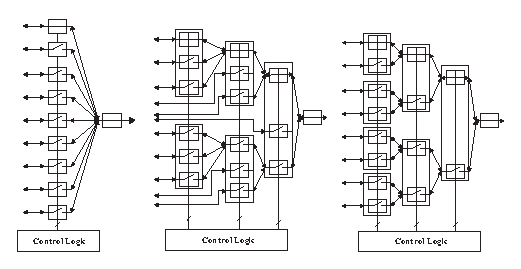
\includegraphics[width=1.0\textwidth]{SIPO_PISO_vet}
		\caption[Arquiteturas de PISO/SIPO]{Arquiteturas de PISO/SIPO (retirada de \cite{R012})}
		\label{fig:PISO-SIPO}
	\end{center}
\end{figure}

No circuito mais á esquerda, denominada de a) pelo autor de \cite{R012}, visualiza-se uma estrutura de um único andar, todavia esta é demasiado lenta devido às capacidades intrínsecas largas no nó de conversão. No circuito do centro, b), é representada uma topologia  heterogénea que se torna mais rápida que a apresentada em a). Já no último circuito apresentado na figura (o da mais à direita), c), é representada uma topologia em árvore binária que é a mais rápida segundo o autor de \cite{R012}. O autor reforça ainda a ideia de que a utilização de multiplexadores de 2:1 e 1:2 são muito importantes para se obter uma arquitetura de funcionamento rápido. É de notar ainda que quando se utiliza uma arquitetura de serialização/deserialização em árvore binária, tal como o autor sugere, as portas de entrada do serializador terão dezenas de entradas, tal como as portas de saída do deserializador terão dezenas de saída, e por isso alguns pontos que necessitam de circuitos de velocidade elevada e outros não. Para tal é necessário ter em atenção que tipo de circuitos são usados em cada etapa do serializador, dada a sua necessidade de velocidade.

Em situações em que as taxas de débito são muito elevadas a utilização de \textit{shift registers} torna-se também bastante eficiente para implementar um serializador/deserializador. Na figura \ref{fig:piso} é possível visualizar o exemplo de uma serializador com a base em\textit{ shift-register} de 4 bits e na figura \ref{fig:sipo} um deserializador com base na mesma arquitetura de 4 bits.

	\begin{figure}[h!]
	\begin{center}
		\leavevmode
		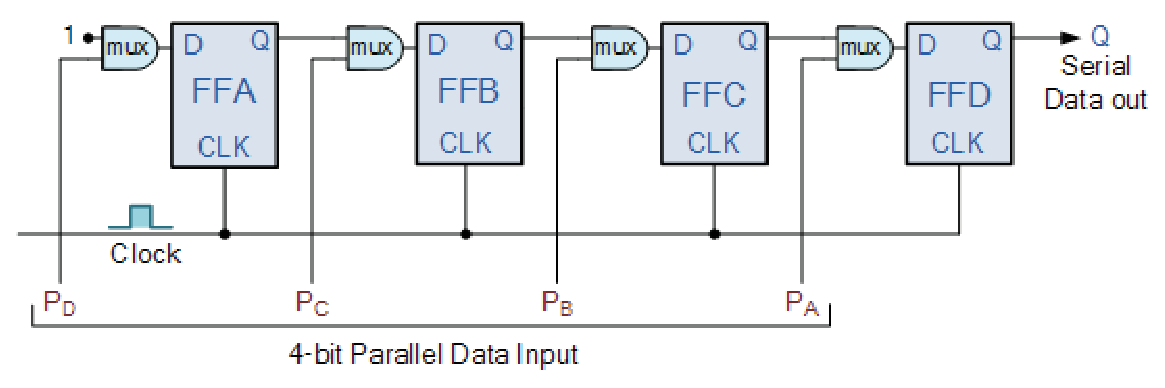
\includegraphics[width=0.8\textwidth]{PISO}
		\caption[Arquitetura de um \textit{shift-register} serializador de 4 bits]{Arquitetura de um \textit{shift-register} serializador de 4 bits (retirado de \cite{R034})}
		\label{fig:piso}
	\end{center}
\end{figure}

O serializador lê os dados os dados em paralelo a um sinal de relógio cuja frequência é mais baixa e após serem lidos (quando o sinal de escrita na arquitetura estiver desligado) os sinais saem à cadência de um sinal de relógio múltiplo superior ao anteriormente mencionado, obtendo-se desta maneira um sinal em série de alta velocidade.

	\begin{figure}[h!]
	\begin{center}
		\leavevmode
		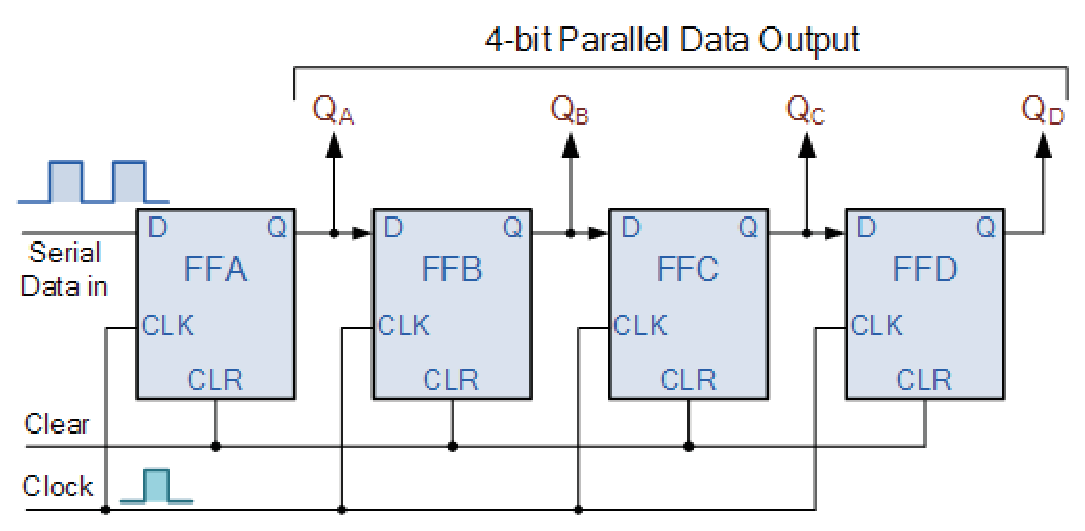
\includegraphics[width=0.8\textwidth]{SIPO}
		\caption[Arquitetura de um \textit{shift-register} deserializador de 4 bits]{Arquitetura de um \textit{shift-register} serializador de 4 bits (retirado de \cite{R034})}
		\label{fig:sipo}
	\end{center}
\end{figure}


No caso do deserializador apresentado na figura \ref{fig:sipo}, e segundo a fonte \cite{R034}, os dados que chegam em série a uma frequência determinada pelo sinal de relógio \textit{clock}, são movidos do registo A para o B e de seguida para o C e por fim para o D a essa mesma frequência (que corresponde à frequência de transmissão em série). Nas saídas QA, QB, QC e QD obtêm-se esses sinais, que chegaram ao início da cascada de registos em série, em paralelo fazendo a sua amostragem a uma frequência mais baixa (múltipla da mais alta, tal como acontecia no serializador).

\begin{figure}[h!]
	\begin{center}
		\leavevmode
		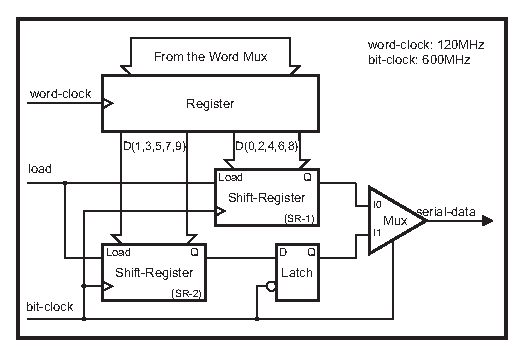
\includegraphics[width=0.75\textwidth]{exemplo_serializer}
		\caption[Exemplo de um serializador de 10 bits]{Exemplo de um serializador de 10 bits (retirado de \cite{R033})}
		\label{fig:exemplo_de_33}
	\end{center}
\end{figure}

Os autores de \cite{R033} utilizam este tipo de estrutura de serializador para obter uma ligação em série de \SI{1.25}{\giga\bit\per\second}. A arquitetura em questão é apresentada na figura \ref{fig:exemplo_de_33}.

Neste caso em específico, a cada ciclo de relógio de "\textit{word-cycle}" é lida uma palavra de 10 bits proveniente de um multiplexador para um registo com nome na figura de "\textit{Register}". A saída deste modulo é então dividida em dois "\textit{shift-register}"  de 5 bits cada. Tal como a figura ilustra, os bits são separados de forma a que bits adjacentes entrem em \textit{shift-registers} diferentes. A saída do primeiro \textit{shift-register} é a entrada do multiplexador de saída, enquanto que a saída do segundo \textit{shift-register} é a entrada de uma \textit{latch} que serve exatamente para atrasar meio ciclo de relógio a operação de alternação de registos em relação ao primeiro \textit{shift-register}. As saídas do multiplexador de saída são selecionadas pela alternância do sinal de relógio com frequência mais elevada, fazendo assim uma correta seleção entre os bits adjacentes e obtendo a saída com a velocidade pretendida para este caso em específico: \SI{1.25}{\giga\bit\per\second}. Este exemplo é aqui mencionado para que se possa perceber como é possível tirar partido deste tipo de arquiteturas de serialização.
%
%The output of one of the shift-registers (SR-1) drives one input of the output multiplexer while the other one (SR-2) drives a latch. This latch drives the other multiplexer input and its purpose is to delay the data shifting operation by half a clock cycle in relation to the output of the first SR. Since the select input of the output multiplexer is driven by the shifting clock (600MHz), it correctly selects between adjacent bits and constructs the desired 1.2Gbit/s bit stream. This is represented schematically in the timing diagram of Figure 3.


Para que estes blocos funcionem é necessário que exista um sinal de relógio de alta frequência (à taxa de débito do canal em série) e um sinal de baixa frequência também (para a os dados em paralelo). O sinal de relógio mais alto é usado para amostrar na saída os dados provenientes do sinal em paralelo e ao mesmo tempo para amostrar os dados recebidos em série. O sinal de frequência mais baixo, é utilizado para colocar na saída os dados que são amostrados do sinal em série. Deste modo, é necessário a utilização de multiplicadores de sinal de relógio e divisores de frequências.


\subsubsection*{Interfaces com a camada física} \label{subsub:pre_enfase_equalizacao}

As interfaces com as camadas físicas em ambos os lados da transmissão (recetor e transmissor) incluem circuitos analógicos que permitem transmitir e receber sinais diferenciais. Contudo o sinal comunicado ao longo do canal pode sofrer interferências por vários motivos, interferências essas que são críticas no que toca à receção do sinal. Por isso existe uma necessidade de utilizar técnicas que melhorem a ligação entre os dois terminais. Segundo \cite{R012}, esta melhoria poderia ser facilmente obtida através da utilização de canais de ligação de melhor qualidade. No entanto esta opção traz custos acrescidos à ligação. 

Assim sendo, recorre-se a técnicas implementadas nestas mesmas interfaces que por um lado são responsáveis por "preparar" os sinais a serem transmitidos para um canal ruidoso, precavendo a sua alteração, e por outro são responsáveis de corrigir os dados recebidos de acordo com determinadas características. Estas técnicas que estão aqui a ser mencionadas têm o nome de pré-ênfase do lado do transmissor e equalização do lado do recetor e passarão a ser descritas com mais detalhe.

%Pré-Enfase:
%--> o que acontece no canal para que esta seja necessária
Durante a transmissão no canal físico é normal haver o fenómeno de interferência inter-simbólica que ocorre devido ao facto de haver longos períodos de transmissão de um determinado valor, seguido de um curto período de tempo com um valor oposto. Segundo a fonte \cite{R032}, o meio físico tem menos tempo para carregar o valor que é transmitido no curto período de tempo e por isso acaba por produzir uma amplitude mais baixa.
\begin{figure}[h!]
	\begin{center}
		\leavevmode
		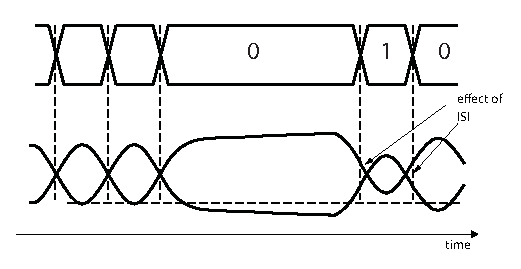
\includegraphics[width=0.75\textwidth]{ISI_vet}
		\caption[Efeito da Interferência Inter-Simbólica numa transmissão]{Efeito da Interferência Inter-Simbólica numa transmissão (adaptada de \cite{R032})}
		\label{fig:isi}
	\end{center}
\end{figure}
Para melhor entendimento, a figura \ref{fig:isi} ilustra o fenómeno de interferência inter-simbólica. Considere-se a transmissão de cima da figura o sinal efetivamente transmitido, e a transmissão de baixo as distorções que o mesmo sofre no canal. Quando há uma longa transmissão de um determinado valor, na figura ilustrado como 0, e de seguida uma pequena transição do valor oposto então o canal não tem tempo para carregar completamente o valor, sofrendo a distorção que se visualiza na figura. Isto pode vir a causar problemas no recetor no que toca à deteção desta transição distorcida.
%--> o que esta faz

Torna-se evidente a necessidade de controlar este tipo de interferências, e como tal na interface com o canal físico recorre-se à técnica de pré-ênfase. Segundo \cite{R032} esta característica é talvez a  mais importante da interface com a camada física e consiste num \textit{overdriving} (dar um ênfase) intencional no início de uma transição e um \textit{underdriving} nos bits seguintes que apresentem o mesmo valor. Este segundo processo também é conhecido por \textit{de-emphasis}. Desta maneira, quando acontece o fenómeno de interferência inter-simbólica, a capacidade do canal recuperar a total amplitude de uma pequena transição não se tornará um problema.

%--> Concluir a utilização desta técninca e introduzir a outra
Assim sendo, do lado do transmissor é feito um pré-ênfase do sinal mesmo antes do canal de transmissão. Todavia tal não é certamente suficiente para uma correta reconstituição do sinal e o recetor necessita de recorrer a técnicas para a sua correta recuperação.

%Equalização
%--> o que esta faz
No lado do recetor é utilizada a técnica de equalização que vem tentar compensar as distorções que são introduzidas na frequência. Segundo a fonte \cite{R032}, esta técnica divide-se em dois grandes tipos: equalizador ativos e passivos.

Um equalizador passivo é um circuito passivo que tem uma resposta em frequência complementar as perdas da transmissão, podendo ser equiparado a um filtro. Isto porque efetivamente o que um equalizador passivo faz, segundo a fonte \cite{R032}, acaba por ser filtrar as frequências que a linha de transmissão não passa e não filtrar as que a mesma passa. Por outro lado, os equalizador ativos, podem ser vistos como amplificadores/atenuadores dependentes da frequência. Estes podem ainda ser divididos em dois tipos: equalizadores fixos e adaptativos. Os equalizadores fixos  terão sempre a mesma resposta em frequência de acordo com o padrão que lhes é determinado. Segundo o autores de \cite{R012} e de \cite{R032} um equalizador adaptativo é mais complexo mas também tem mais vantagens comparativamente aos outros tipo de equalizadores.

Um equalizador ativo adaptativo analisa os dados que vão chegando ao recetor e deteta quais são as frequências que estão a ser atenuadas pela linha de transmissão e faz os ajustes necessários de acordo com as medidas que se obtêm realizadas num \textit{loop} fechado. Essencialmente, para tomar uma decisão tem em conta todos os outros dados chegados anteriormente ao sistema. Este tipo de equalizadores são geralmente usados quando há codificações de linha específicas.
%
%\begin{figure}[h!]
%	\begin{center}
%		\leavevmode
%		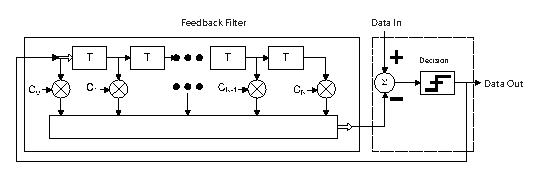
\includegraphics[width=1.0\textwidth]{dfe_vet_1}
%		\caption{Efeito da Interferência Inter-Simbólica numa transmissão, adaptada de \cite{R032}}
%		\label{fig:isi}
%	\end{center}
%\end{figure}

Segundo \cite{R032}, os equalizadores ativos fixos são melhores para sistemas constantes, como por exemplo ligações \textit{chip-to-chip} ou então ligações cujos cabos têm um comprimento fixo. Por outro lado, os equalizadores ativos adaptativos são melhores para ligações inconstantes e até mesmo com comprimento de ligação variável.
%Por outro lado, também pode ser utilizada uma técnica de equalização que consegue obter bons resultados sem custos acrescidos à ligação. Ainda na mesma referência são apresentadas diferentes combinações de métodos de equalização que passam a ser brevemente descritos:
%
%\begin{itemize}
%	\item Linear ou não-linear
%
%	\item Pode ser implementado em tempo contínuo ou discreto
%	\item Pode ser adaptativo ou fixo
%\end{itemize}
%
%Assim sendo, existe um vasto conjunto de opções de equalização que estão diretamente relacionadas com o circuito CDR (\textit{Clock Data Recovery}), sendo que as mais importantes serão referidas mais à frente neste relatório. 


\subsubsection*{Sinalização Física} \label{subsub:sinalizacao_fisica}
%Sinalização Diferencial Vs Sinalização única


A implementação da camada física dos serializadores e deserializadores de alta velocidade tomam uma forma universal baseada em interfaces eletricamente diferenciais, segundo \cite{R032}. Esta forma de transmissão consiste no envio de dois sinais que se complementam eletricamente relativamente a uma massa comum. A principal vantagem que esta metodologia de transmissão acarta consigo é a uma maior rejeição ao ruído em modo-comum uma vez que o sinal no recetor é obtido através da diferença entre as duas tensões dos sinais diferencias recebidos. Assim sendo, este tipo de transmissão torna-se vantajosa quando a interferência eletromagnética (EMI - \textit{Electromagnetic interference} ) ou a interferência de radio-frequência (RFI - \textit{Radio Frequency interference}) se tornam problemáticas na transmissão, pois caso estas existam a sua interferência será aplicada em ambos os sinais (positivo e negativo) e no recetor a diferença será a mesma, não afetando a recuperação dos dados transmitidos.

Os métodos de implementação de sinalização diferencial podem variar em diversas características, como por exemplo o consumo de energia e tipo de aplicações em que podem ser implementadas. O autor de \cite{R032} menciona os três mais comuns:

\begin{itemize}
	\item \textbf{LVDS - \textit{Low-Voltage Differential Signaling}:} é uma técnica que opera a uma baixa potência e que atinge velocidades de transmissão até \SI{3.125}{\giga\bit\per\second}.
	\item \textbf{LVPELC - \textit{Low-Voltage Pseudo Emitter-Coupled Logic}}: é uma técnica que consome entre média e alta potência atingindo velocidades de transmissão superiores a \SI{10}{\giga\bit\per\second}.
	\item \textbf{CML - \textit{Current Mode Logic}:} técnica que consome uma potência de valores médios, atingindo ainda assim velocidades de transmissão superiores a \SI{10}{\giga\bit\per\second}.
\end{itemize}

Os valores de consumo de potência e velocidades de transmissão para cada uma das técnicas apresentadas anteriormente foram retiradas da fonte \cite{R036}. Segundo o autor de \cite{R032} o método mais adequado para implementação em ligações cujas taxas de ligação rondam os \SI{}{\giga\bit\per\second} deve ser a CML.

\subsubsection*{Requisitos de sinais de relógio de referência}

O sinal de relógio de alta frequência é bastante importante na implementação de arquiteturas de serialização e deserialização de alta velocidade, isto porque este sinal é necessário tanto do lado do recetor como do transmissor. Do lado do transmissor é necessário para gerar os símbolos a serem transmitidos e do lado do recetor é necessário para que a amostragem do sinal recebido possa ser bem realizada. Segundo a fonte \cite{R012}, é comum que este sinal de relógio seja partilhado entre o recetor e o transmissor, havendo, contudo, a necessidade de ajuste de fase deste sinal do lado do recetor. Este ajuste de fase deve-se essencialmente por dois motivos: o atraso e ruído do canal. Por um lado, durante a transmissão é introduzido um atraso inerente no sinal que não é conhecido à \textit{priori}, e por outro durante a transmissão também é introduzido ruído que torna a fase do sinal recebido bastante crítica para o desempenho do transcetor. 

Assim sendo,tanto a fonte \cite{R032} como a fonte \cite{R012} reforçam a ideia de que o sinal de alta velocidade de referência possui requisitos muito particulares para o correto funcionamento do transcetor, uma vez que influencia fortemente o seu desempenho. Entre eles destacam-se o baixo ruído, elevada precisão e uma geração contínua do mesmo. Um simples sinal gerado por um oscilador local não é suficiente para cumprir tais critérios, remata o autor de \cite{R012}. Desta maneira, é recomendado o uso de osciladores externos, capazes de serem reprogramados para determinadas frequências no sentido de se obter um sinal mais limpo e preciso. Tal será utilizado neste projeto através de um módulo disponível na FPGA VC7203 que será explicado com mais detalhe mais à frente quando se abordar o trabalho desenvolvido.


\subsubsection*{Importância da criação e uso de pacotes}

O autor de \cite{R032} menciona a importância de criação de "pacotes" que contribuem para a definição do protocolo de transmissão em série. Antes de se perceber que tipos de tramas constituem um pacote é necessário ter em conta que um "pacote" consiste num conjunto de \textit{bytes} bem definidos que contém um cabeçalho, dados e fim do mesmo.

Em qualquer tipo de transmissão de dados são usados pacotes para os transmitir, e a comunicação em série de alta velocidade não pode fugir a esta realidade, porque este tipo de arquiteturas exigem métodos de alinhamento do \textit{stream} de bits chegados em palavras, transmissão de determinados padrões para ser possível a recuperação do relógio entre outros. Assim, é possível aproveitar a necessidade da transmissão destes determinados padrões e criar a partir daqui um pacote de transmissão que sirva para sinalizar as diferentes fases de transmissão dos dados e  ao mesmo tempo permita que o sinal de relógio seja recuperado e os dados alinhados.

Segundo o autor \cite{R032}, o pacote de transmissão deve ter bem definidas determinadas tramas, entre as quais:
\begin{itemize}
	\item \textbf{Inicio de Pacote (\textit{Start of Packet}): }para poder sinalizar a chegada do início de um novo pacote
	\item \textbf{Fim de Pacote (\textit{End of Packet}):} para sinalizar o fim da transmissão de um pacote inteiro
	\item\textbf{Dados :} tramas onde serão transmitidos os dados, pode conter determinados símbolos especiais que indiquem que tipo de dados são transmitidos
	\item \textbf{Símbolo de Espera (\textit{Idle Symbol}):} estas tramas devem ser enviadas sempre que não houver dados para transmitir para garantir que a transmissão contínua dos dados continua alinhada e o sinal de relógio a ser recuperado.
\end{itemize}


\subsubsection*{Correcção do sinal de relógio}
	
Tal como referido anteriormente, a comunicação de sinais de alta velocidade pode sofrer diversas interferências durante a sua transmissão. Contudo, segundo \cite{R012}, após a equalização do sinal estas mesmas interferências são parcialmente compensadas permitindo assim uma recuperação dos dados transmitidos.  Para fazer a correta recuperação do sinal é necessário recorrer a um circuito que recupere o sinal de relógio transmitido do emissor para que este possa ser usado para recuperação dos dados transmitidos. 

\subsubsection*{Deteção de erros na transmissão}

Durante a transmissão em série de alta velocidade, e tal como já foi indicado anteriormente, são introduzidos ruídos e distorções nos sinais e apesar das diversas técnicas já apresentadas anteriormente que evitam estes erros existem códigos detetores e corretores de erros que podem ainda ser aplicados.
No caso em específico deste projeto em que se trata da transmissão em série de dados de imagem e som, o mais conveniente é a implementação de códigos apenas detetores de erros, pois não traz vantagem ao projeto corrigir esses mesmos erros detetados, por muito curto que seja o tempo que tal processo demore. O autor de \cite{R012} menciona mesmo que uma das técnicas mais utilizadas é o CRC (\textit{Cyclic Redundancy Codes}) e que existem já algumas arquiteturas de serialização/deserialização que incluem esta mesma técnica, e como tal esta será brevemente abordada. 

O principal objetivo desta técnica é determinar se o sinal que foi transmitido pelo canal com ruído foi corrompido ou não durante a transmissão. Segundo \cite{R028}, a ideia básica por trás deste algoritmo de deteção de erros é tratar a mensagem a ser transmitida como um número binário normal, dividir por um número binário fixo e o resto dessa mesma divisão será o \textit{checksum}\footnote{Código usado para verificar a integridade dos sinais transmitidos em canais ruidosos} da mensagem, enviado na mesma trama. Do lado do recetor é aplicado o mesmo algoritmo à trama recebida e de seguida verifica-se se o resto da divisão corresponde ao \textit{checksum} recebido. No pior dos casos quando o \textit{checksum} não corresponder à mensagem recebida então perderá-se a transmissão de um pacote (no caso do projeto será uma imagem).

Ainda segundo a fonte \cite{R028}, o que torna este algoritmo mais fiável relativamente aos outros é a complexidade de determinação do \textit{checksum}. Outros algoritmos semelhantes podem receber um \textit{checksum} corrompido e uma mensagem também corrompida, mas devido à falta de robustez do mesmo, apresentam consistência entre o \textit{checksum} e a mensagem, não detetando nenhum erro. No entanto, como o CRC é um algoritmo mais complexo, tal não acontece, tornando-o num código detetor de erros robusto e que por isso pode ser utilizado neste projeto em concreto.

\section{Saídas em série de alta velocidade da FPGA VC7203}

A FPGA VC7203 disponibiliza de uns transcetores de alta velocidade que devido às suas características são utilizados neste projeto. Esta secção aborda quais as características disponíveis e como podem ser utilizadas no projeto.


\subsection{Localização dos transcetores na FPGA}

As FPGA de série 7 da \textit{Xilinx} têm disponíveis transcetores capazes de comunicação em série de alta velocidade, tal como é necessário neste projeto. Em específico, segundo \cite{R010}, na FPGA XILINX VC7203 Virtex-7 estão disponíveis transcetores GT\footnote{\textit{Gigabit Transceiver}}X que permitem uma velocidade de \SI{12.5}{\giga\bit\per\second} e que são os mais adequados para este projeto. Noutros modelos existem outros transcetores, como por exemplo GTZ (que permite até \SI{28}{\giga\bit\per\second}), GTH (que permite débitos até \SI{13.1}{\giga\bit\per\second}) e GTP (com débitos até \SI{6.6}{\giga\bit\per\second}). No entanto apenas serão abordados os transcetores GTX, visto que são os mais adequados para este tipo de comunicações e os únicos disponíveis na FPGA utilizada. 

Na figura \ref{fig:loc_gtx} é possível visualizar a FPGA a ser utilizada no projeto e visualiza-se ainda assinaladas as entradas GTX (QUAD\_111, QUAD\_112, QUAD\_113, QUAD\_114, QUAD\_115, QUAD\_116, QUAD\_117, QUAD\_118 e QUAD\_119).
 
\begin{figure}[h!]
	\begin{center}
		\leavevmode
		\includegraphics[width=0.9\textwidth]{loc_gtx_vet}
		\caption[Localização física na FPGA dos GTX]{Localização física na FPGA dos GTX (retirada de \cite{R008})}
		\label{fig:loc_gtx}
	\end{center}
\end{figure}

\subsection{Arquitetura dos transcetores} \label{sub:arqGTX}

Cada GTX é composto por quatro transmissores e quatro recetores. É possível visualizar o conector do GTX na figura \ref{fig:gtx_fis} . A figura A corresponde ao conector e a figura B faz as correspondência de cada pino do conector. Através da figura B é possível verificar que efetivamente existem quatro pares diferencias de transmissores/recetores e ainda dois pares diferenciais que são usados para conectar os sinais de relógio de referência. Nestes conectores são ligados cabos SMA(\textit{SubMiniature version A}) diferenciais.

\begin{figure}[h!]
	\begin{center}
		\leavevmode
		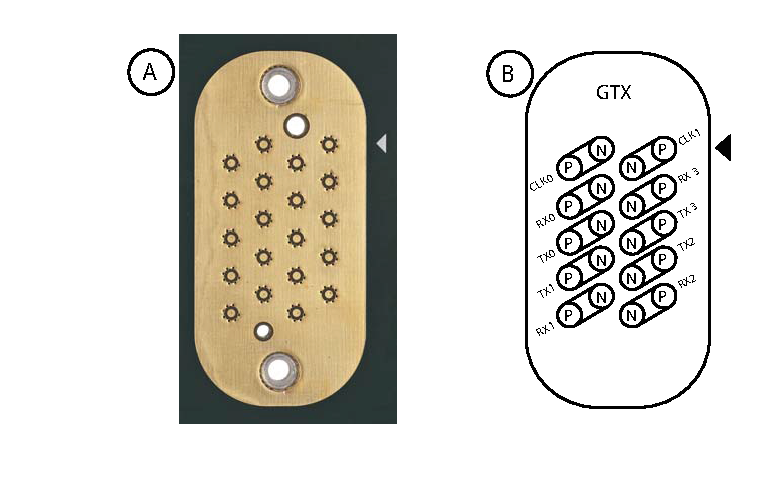
\includegraphics[width=0.75\textwidth]{gtx_fisico}
		\caption[Conectores GTX localizados na FPGA]{Conectores GTX localizados na FPGA (retirada de \cite{R008})}
		\label{fig:gtx_fis}
	\end{center}
\end{figure}

Apesar de em cada GTX estarem disponíveis quatro transmissores/recetores, o projeto apenas faz uso de um canal para efetuar a transmissão de dados. Na figura \ref{fig:gtx_geral_arq} é apresentada uma arquitetura geral dos transcetores da FPGA.

\begin{figure}[h!]
	\begin{center}
		\leavevmode
		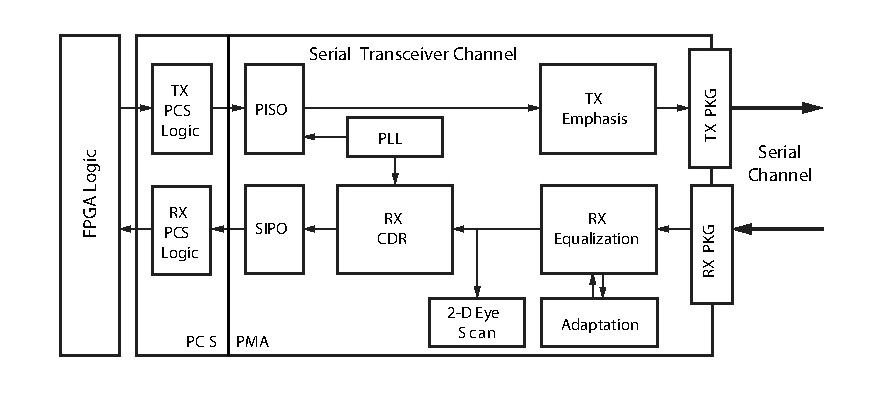
\includegraphics[width=1.0\textwidth]{geral_arq_trans}
		\caption[Arquitetura geral dos transcetores]{Arquitetura geral dos transcetores (retirada de \cite{R010})}
		\label{fig:gtx_geral_arq}
	\end{center}
\end{figure}


A arquitetura dos mesmos passa a ser brevemente descrita, segundo \cite{R010} e \cite{R011}:
\begin{itemize}
	\item \textbf{Módulo PMA (\textit{Physical Medium Attachment Sublayer})} que inclui:
	\begin{itemize}
		\item Bloco série/parelo e vice-versa (PISO e SIPO).
		\item PLL (\textit{Phase-locked loop)}.
		\item CDR (\textit{Clock Data Recovery}).
		\item Pré-Ênfase e Bloco de Equalização.
		\item Suporta uma taxa de débito de saída até \SI{12.5}{\giga\bit\per\second}.
		\end{itemize}
	\item \textbf{Módulo PCS (\textit{Physical Coding Sublayer}) que inclui:}
	\begin{itemize}
		\item Lógica de processamento dos dados em paralelo reconfigurável
		\item \textit{Datapath} de 2 e 4 \textit{byte} internos para suportar diferentes taxas de débitos
		\item Codificação e descodificação 8B/10B
		\item Deteção de vírgula e alinhamento de palavra
		\item PRBS (\textit{Pseudo Random Bit Sequence}) gerador e verificador
		\item FIFO para correção do sinal de relógio e ligação do canal
		\item Este bloco trabalha com taxas de débitos de informação mais baixas.
	\end{itemize}
	\item \textbf{Interface com a lógica da FPGA.}
	\item \textbf{Interface com o canal físico em série diferencial.}
\end{itemize}

O transmissor e o recetor funcionam separadamente apesar de na figura \ref{fig:gtx_geral_arq} sugerir que funcionam em conjunto. Estes dispõe de blocos necessários referidos em \ref{sec:conexaoSerie} e como tal são usados no projeto. Mais detalhes sobre o funcionamento independente do transmissor e recetor serão detalhados quando for abordado o trabalho desenvolvido sobre a comunicação em série.


%\begin{figure}[h!]
%	\begin{center}
%		\leavevmode
%		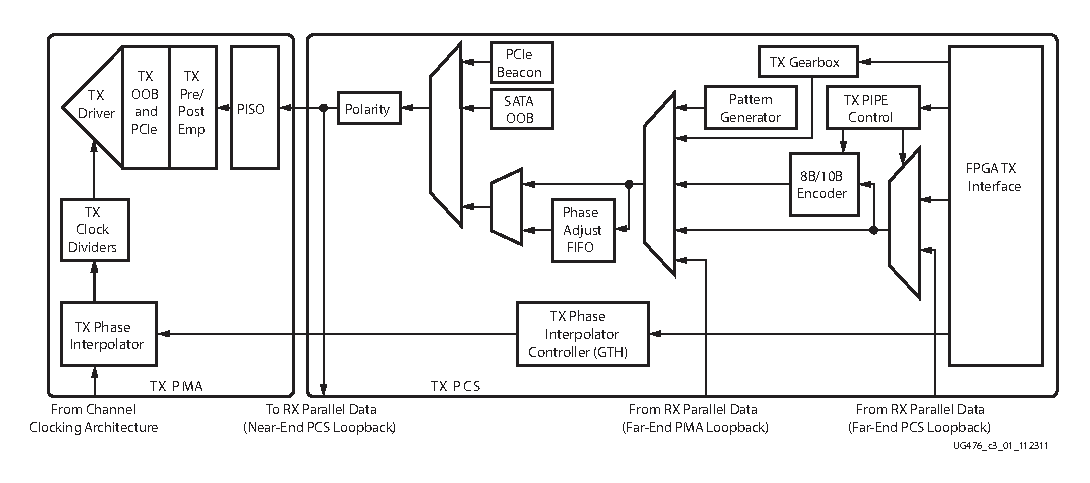
\includegraphics[width=1.0\textwidth]{tx_gtx_arq}
%		\caption{Arquitetura do transmissor GTX disponibilizada na FPGA , retirada de \cite{R011}}
%		\label{fig:rx_gtx}
%	\end{center}
%\end{figure}

%\subsection{Recetor}

%\begin{figure}[h!]
%	\begin{center}
%		\leavevmode
%		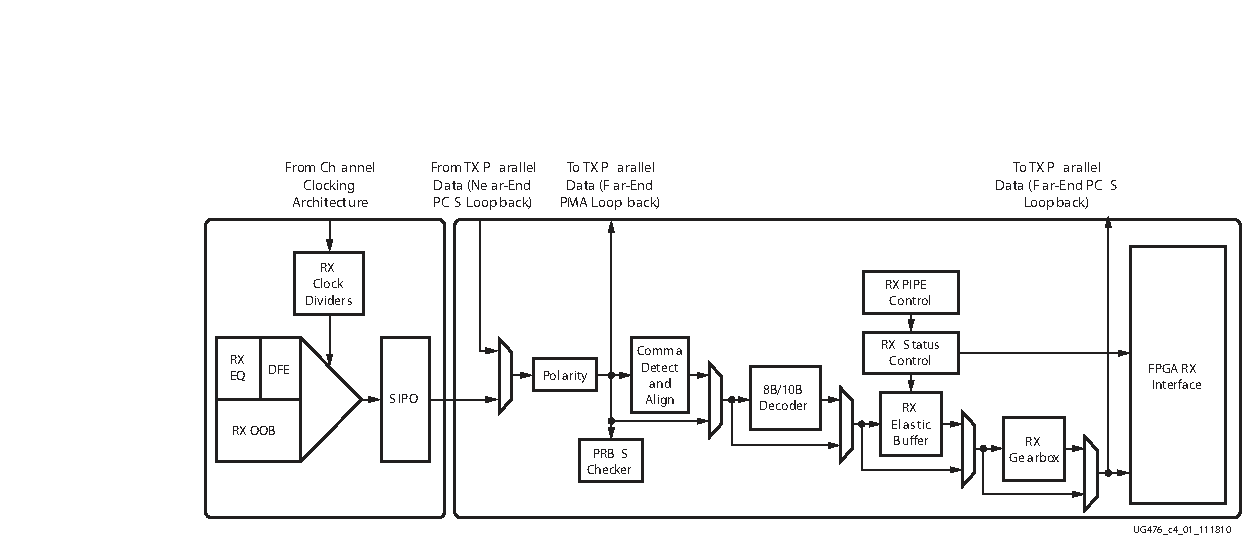
\includegraphics[width=1.0\textwidth]{rx_gtx_arq}
%			\caption{Arquitetura do recetor GTX disponibilizada na FPGA , retirada de \cite{R011}}
%		\label{fig:rx_gtx}
%	\end{center}
%\end{figure}
\section{Sincronização entre diferentes domínios de relógio} \label{sec:sincronizacao}

Tal como referido em \ref{sec:descrição_objetivos} o projeto está dividido em duas partes fundamentais: a primeira em que se trabalha apenas com os dados provenientes do sinal HDMI, e uma segunda parte que conjugará dois domínios de sinais de relógio (do HDMI e do GTX). A figura \ref{fig:dominios_diferentes} ilustra os diferentes domínios de relógio existentes no projeto.

\begin{figure}[h!]
	\begin{center}
		\leavevmode
		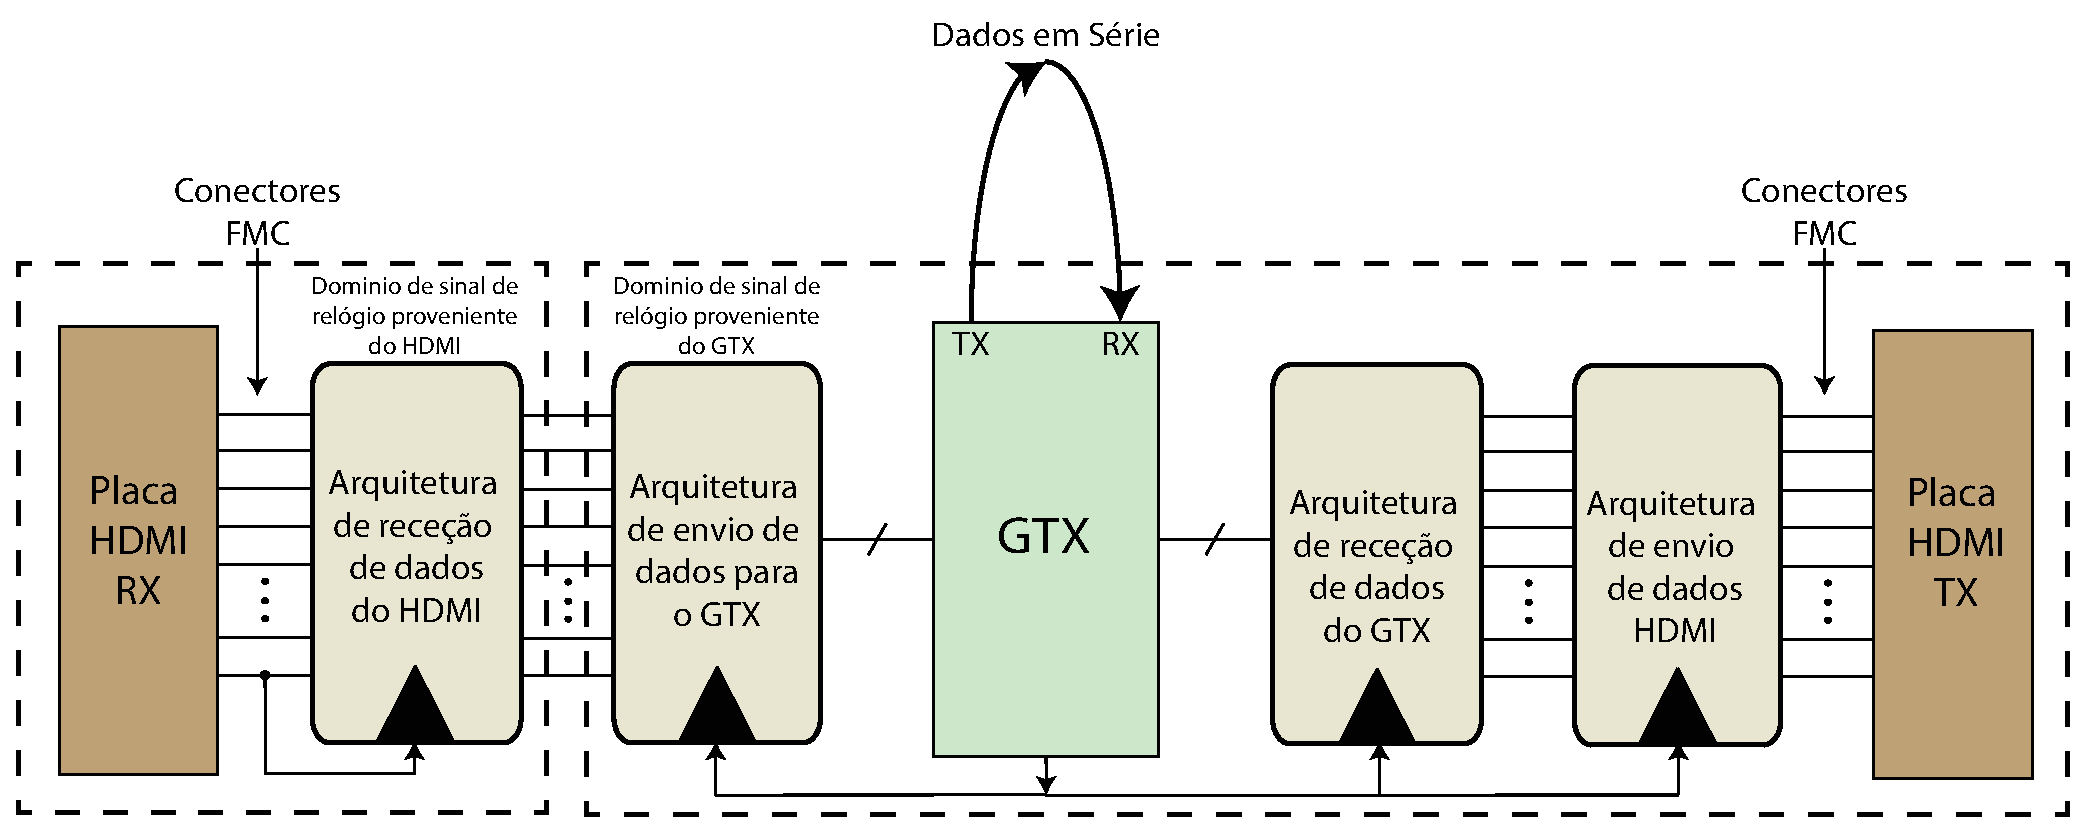
\includegraphics[width=1.0\textwidth]{diagrama_dominios}
		\caption{Representação dos diferentes domínios de sinais de relógio no projeto}
		\label{fig:dominios_diferentes}
	\end{center}
\end{figure}

A placa HDMI RX e a arquitetura de receção de dados HDMI funcionam a um sinal de relógio proveniente da placa HDMI. Todavia a arquitetura responsável pelo envio dos dados para o GTX e posterior receção dos dados provenientes do mesmo funciona a um sinal de relógio proveniente do GTX. Também a arquitetura responsável pelo envio dos dados para a placa HDMI funciona a esse mesmo sinal de relógio proveniente do GTX (tal será explicado quando for abordado o trabalho referente à segunda parte do trabalho). Assim sendo, existem aqui dois principais domínios de relógio diferentes o que pode vir a provocar falta de sincronização entre a transição de dados de um para outro.


Ora, segundo a fonte \cite{R024} e \cite{R037}, este problema pode levar a captação de dados que se encontram num estado de meta-estabilidade e estes propagam-se ao longo do sistema o que certamente causará danos irreversíveis na transmissão de dados. 

Para se perceber o problema de meta-estabilidade é necessário ter em consideração que os dispositivos digitais têm determinados requisitos temporais que necessitam de ser cumpridos para que possam captar corretamente os dados. Esses requisitos passam de seguida a ser enumerados tal como em \cite{R037}:

\begin{itemize}
	\item \textbf{Tempo de \textit{Set Up} (T{\tiny SU})}: Tempo mínimo em que a entrada do registo deve estar estável antes da subida positiva do sinal de relógio.
	\item \textbf{Tempo de \textit{Hold} (T{\tiny H})}: Tempo mínimo em que a entrada do registo deve estar estável depois da subida positiva do sinal de relógio.
	\item \textbf{Tempo de \textit{clock-to-output} (T{\tiny CO})}: Tempo necessário para o valor estar disponível na saída do registo.
\end{itemize}
 
Quando alguma transição viola o T{\tiny SU} ou T{\tiny H} então a saída não conseguirá obter um valor e ficará num estado de meta-estabilidade, que nem é 0 nem 1. Estes problemas normalmente acontecem em situações em que os dados são transmitidos entre domínios de relógio diferentes, tal como acontece neste projeto, e podem propagar-se no sistema. A figura \ref{fig:metaestabilidade} ilustra este problema.

\begin{figure}[h!]
	\begin{center}
		\leavevmode
		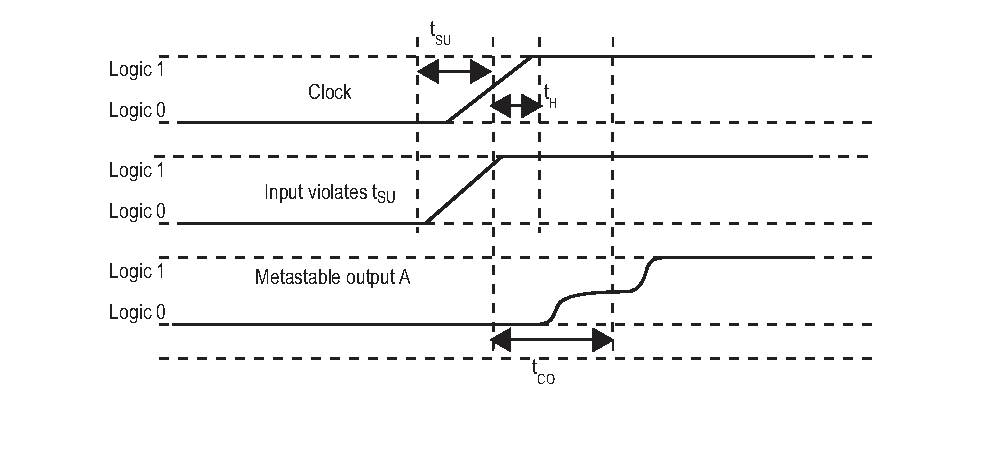
\includegraphics[width=1.0\textwidth]{meta_stable}
		\caption[Exemplo de metaestabilidade]{Exemplo de metaestabilidade (adaptado de \cite{R037})}
		\label{fig:metaestabilidade}
	\end{center}
\end{figure}

Visto que é possível prever antecipadamente que este tipo de problemas ocorrerão durante o desenvolvimento do projeto, é então necessário levá-los em conta e procurar métodos que os possam resolver.

Segundo \cite{R037} e \cite{R024}, para a correção de problemas de meta-estabilidade são tipicamente usadas cadeias de registos de sincronização no domínio de relógio de destino para que o sinal seja re-sincronizado nesse mesmo domínio. Isto permitirá que os registos tenham mais tempo para resolver eventuais estados de meta-estabilidade para um valor estável antes do valor ser usado no domínio de destino.  O tempo disponível entre os caminhos de registo para registo é o tempo disponível para o sinal metaestável estabilizar. A figura \ref{fig:sincronizacao} ilustra uma cadeia de registos de sincronização.


\begin{figure}[h!]
	\begin{center}
		\leavevmode
		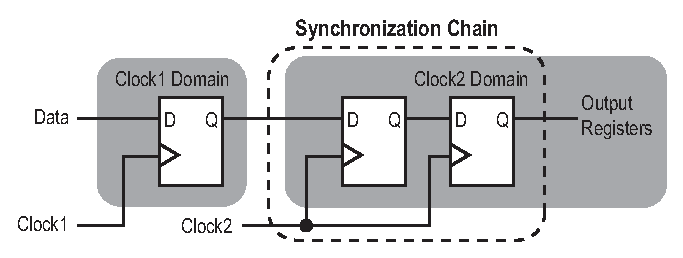
\includegraphics[width=0.8\textwidth]{sincronizacao_vet}
		\caption[Exemplo de cadeia de registos de sincronização]{Exemplo de cadeia de registos de sincronização (retirado de \cite{R037})}
		\label{fig:sincronizacao}
	\end{center}
\end{figure}

Segundo \cite{R037}, a cadeia de registos de sincronização funciona da seguinte maneira: todos os registos devem trabalhar ao mesmo sinal de relógio (do domínio de destino) e os registos devem enviar os dados apenas para um único registo na cadeia, excepto o último. Para além disso o primeiro registo da cadeia tem como entrada um sinal proveniente de um domínio de sinal de relógio assíncrono com o de destino.

Assim sendo, a utilização desta técnica virá prevenir eventuais problemas de sincronização que possam vir a existir entre diferentes domínios de relógio existentes no projeto.